\fenicschapter{Improved Boussinesq Equations for Surface
  Water Waves} {Improved Boussinesq Equations for Surface
  Water Waves} {Nuno D. Lopes, Pedro J. S. Pereira and
  L. Trabucho} {lopes}

%\editornote{Move macros to common macros after deciding what
%  to do about bold fonts.}

%\editornote{List authors with  full names}

%{{{ Abstract
The main motivation of this work is the implementation of a
general solver for some of the improved Boussinesq
models\index{Boussinesq models}.  Here, we use an extension
of the model proposed by~\cite{ZhaoTengCheng2004} to
investigate the behavior of surface water waves. The
equations in this model do not contain spatial derivatives
with an order higher than 2. Some effects like surface
tension, energy dissipation and wave generation by natural
phenomena or external physical mechanisms are also included.
As a consequence, some modified dispersion relations are
derived for this extended model.
%}}}

%{{{ Overview
\section{Overview}
The \fenics project, via \dolfin, \ufl and \ffc, provides
good technical and scientific support for the implementation
of large scale industrial models. Specifically, all the
finite element matrices and vectors are automatically
generated and assembled by \dolfin\ and \ffc, directly from
the variational formulation of the problem which is declared
using \ufl. Moreover, \dolfin\ provides a user friendly
interface for the libraries needed to solve the finite
element system of equations.

We implement a solver for some of the Boussinesq type
systems to model the evolution of surface water
waves\index{water waves} in a variable depth seabed.  This
type of model is used, for instance, in harbor
simulation\footnote{See Fig.~\ref{fig:lopes:harbor} for an
example of a standard harbor.}, tsunami generation and wave
propagation as well as in coastal dynamics.
\begin{figure}
\begin{center}
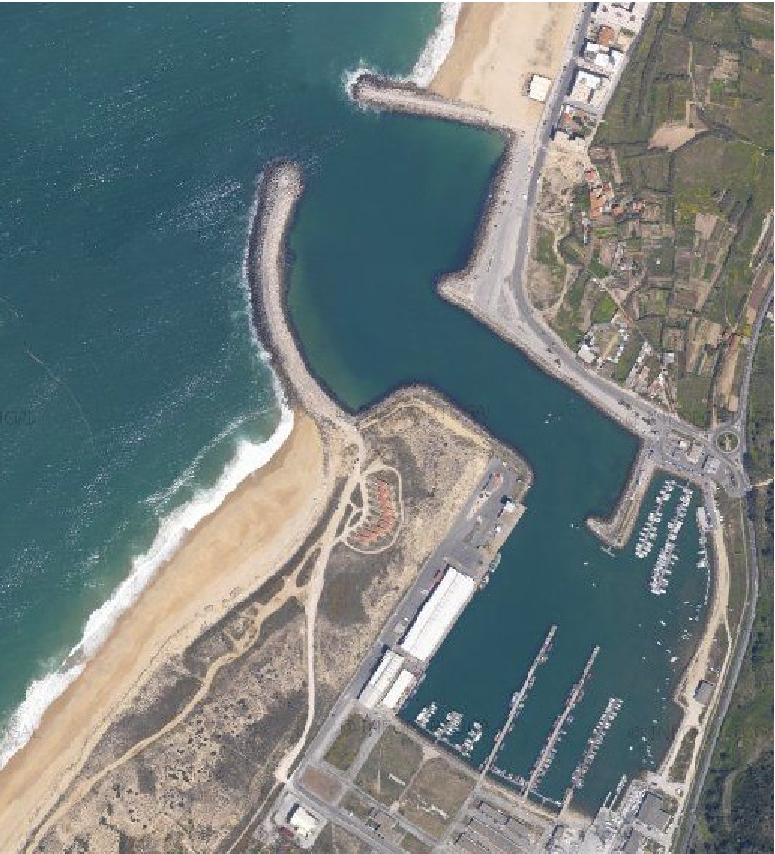
\includegraphics[width=\smallfig]{chapters/lopes/pdf/nazare1.pdf}
\end{center}
\caption{Nazar\'{e}'s harbor,
  Portugal.}\label{fig:lopes:harbor}
\end{figure}

\editornote{Need to get permission for this figure!}

In section~\ref{sec:lopes:dolfwave}, we begin by describing
the DOLFWAVE application, i.e., a \fenics based
application for the simulation of surface water waves (see
the web pages {\tt
http://www.fenicsproject.org/wiki/DOLFWAVE} and {\tt
http://ptmat.fc.ul.pt/$\sim$ndl/}).

The governing equations for surface water waves are
presented in section~\ref{sec:lopes:modelderivation}. From
these equations different types of models can be derived.
There are several Boussinesq models and some of the most
widely used are those based on the wave surface Elevation
and horizontal Velocities formulation (BEV) (see, e.g.,
~\cite{LiuWoo2004}, ~\cite{WalkleyBerzins2002}).
However, we only consider the wave surface Elevation and velocity
Potential (BEP) formulation.  Thus, the number of unknowns
is reduced from five (the three velocity components, the
pressure and the wave surface elevation) in the BEV models
to three (the velocity potential, the pressure and the wave
surface elevation) in the BEP models.  Two different types
of BEP models are taken into account:
\begin{itemize}
\item[{\it i})] a standard  model containing sixth-order
  spatial derivatives;
\item[{\it ii})] the  model proposed by
  ~\cite{ZhaoTengCheng2004} (ZTC), containing only first and
  second-order spatial derivatives.
\end{itemize}
A standard technique is used in order to derive the
Boussinesq-type model mentioned in {\it i)}.  In the
subsequent sections, only the ZTC-type model is considered.
Note that these two models are complemented with some extra
terms, due to the inclusion of effects like energy dissipation,
surface tension and wave generation by moving an impermeable
bottom or using a source function.

An important characteristic of the extended ZTC model,
including dissipative effects, is presented in
section~\ref{sec:lopes:dispersionproperties}, namely, the
dispersion relation.

In sections~\ref{sec:lopes:wavegeneration}
and~\ref{sec:lopes:boundaryconditions}, we describe several
types of wave generation, absorption and reflection
mechanisms.  Initial conditions for a solitary wave and a
periodic wave induced by Dirichlet boundary conditions are
also presented.  Moreover, the extended ZTC model includes a
source function to generate surface water waves, as proposed
in~\cite{WeiKirbySinha1999}.  Total reflective walls are
modelled by standard zero Neumann conditions for the wave
surface elevation and velocity potential.  The wave energy
absorption is simulated using sponge layers.

Section~\ref{sec:lopes:numericalmethods} is dedicated to the
numerical methods used in the discretization of the
variational formulation.  The discretization of the spatial
variables is accomplished with Lagrange $P_1$ or $P_2$
finite elements (see Chapter~\ref{chap:kirby-6}) whereas the
time integration is implemented using Runge--Kutta and
predictor-corrector algorithms.

In section~\ref{sec:lopes:numericaltests}, the extended ZTC
equations are used to model three different physical
problems: the evolution of a solitary wave passing through a
submerged bar; the evolution of a periodic wave in a harbor
geometry like that one represented in
Fig.~\ref{fig:lopes:harbor} and the generation of a wave due
to an object moving on a horizontal bottom.  We also use the
first numerical test to illustrate the usage of the DOLFWAVE
application.
%}}}

%{{{ DOLFWAVE overview
\section{DOLFWAVE}\label{sec:lopes:dolfwave}
The main goal of DOLFWAVE is to provide a framework for the
analysis, development and computation of models for surface
water waves, based on finite element methods.  We have
already implemented solvers for the following cases:
\begin{itemize}
\item[{\it i)}] Shallow water wave models for unidirectional
  long waves in one horizontal dimension;
\item[{\it ii)}] Boussinesq-type models for moderately long
  waves with small amplitude in shallow water.
\end{itemize}
The shallow water wave models implemented and mentioned in {\it i)} are the following:
\begin{itemize}
\item The Korteweg--de Vries (KdV) model which consists of a
  weakly nonlinear and dispersive third-order partial
  differential equation for the wave surface elevation. The
  discretization of the spatial variable is accomplished
  using a continuous/discontinuous finite element method
  with Lagrange $P_2$ elements;

\item The Benjamin--Bona--Mahony model, also known as the
  regularized long-wave (RLW) model, which is an improvement
  of the KdV model regarding the dispersive properties.  The
  equation in the RLW model contains only second-order
  spatial derivatives. The discretization of the
  spatial variable is accomplished using continuous finite
  element methods with Lagrange $P_1$ or $P_2$ elements.
\end{itemize}
For the Boussinesq-type models we considered the following
cases:
\begin{itemize}
\item The extended Zhao et al. (ZTC) model which is based on
  a system of two second-order partial differential
  equations for the wave surface elevation and a velocity
  potential. The discretization of the spatial variables is
  accomplished using continuous finite element methods with
  Lagrange $P_1$ or $P_2$ elements;

 \item An extension of the model by \cite{ChenLiu1994} in
   order to include dissipative effects, several forms of
   wave generation and improved dispersive properties.  This
   model is based on a system of two fourth-order partial
   differential equations for the wave surface elevation and
   a velocity potential. The discretization of the spatial
   variables is accomplished using the
   continuous/discontinuous finite element method with
   Lagrange $P_2$ elements
   (see~\cite{LopesPereiraTrabucho}).
\end{itemize}

A predictor-corrector scheme with an initialization
provided by an explicit Runge--Kutta method is used for the
time integration of the equations. We use \ufl\ for the
declaration of the finite element discretization of the
variational forms related to the models mentioned above (see
the \ufl\ form files in the following directories of the
DOLFWAVE code tree: {\tt dolfwave/src/1hd1sforms}, {\tt
dolfwave/src/1hdforms} and {\tt dolfwave/src/2hdforms}).
These files are compiled using \ffc to generate the C++ code
of the finite element discretization of the variational
forms (see Chapter~\ref{chap:alnes-1}).  DOLFWAVE is based
on the C++ interface of DOLFIN $0.9.9$ to assemble and solve
all the systems of equations related with the finite element
method.

All the DOLFWAVE code is available for download at {\tt
https://launchpad.net/dolfwave}.  Some tools for the
generation of the C++ code for boundary conditions and
source functions are included. Scripts for visualization
and data analysis are also part of the application. The
Xd3d post-processor is used in some cases (see {\tt
http://www.cmap.polytechnique.fr/$\sim$jouve/xd3d/}).
DOLFWAVE has a large number of demos covering all the
implemented models (see {\tt dolfwave/demo}). Different
physical effects are illustrated.  All the numerical
examples in this work are included in the demos.
%}}}

%{{{ Model derivation
\section{Model derivation}\label{sec:lopes:modelderivation}
We consider the following set of equations for the
irrotational flow of an incompressible and inviscid fluid:
\begin{subequations}\label{eq:lopes:euler}
\begin{align}
&\displaystyle\frac{\partial u}{\partial t}+\nabla u \cdot
  u=-\nabla\left(\frac{P}{\rho} +g\,
  z\right),\label{eq:lopes:euler-a} \\ &\nabla\times
  u={0},\label{eq:lopes:euler-b}
  \\ &\nabla\cdot{u}=0,\label{eq:lopes:euler-c}
\end{align}
\end{subequations}
where $u$ is the velocity vector field of the fluid, $P$ the
pressure, $g$ the gravitational acceleration, $\rho$ the
mass per unit volume, $t$ the time and the differential
operator
$\nabla=\left(\frac{\partial }{\partial x},\frac{\partial
}{\partial y},\frac{\partial }{\partial z}\right).$ A
Cartesian coordinate system is adopted with the horizontal
$x$ and $y$-axes on the still water plane and the $z$-axis
pointing vertically upwards (see
Fig.~\ref{fig:lopes:schematic}).  The fluid domain is
bounded by the bottom seabed at $z=-h(x,y,t)$ and the free
water surface at $z=\eta(x,y,t)$.
In Fig.~\ref{fig:lopes:schematic}, $L$, $A$ and $H$ are the
characteristic wave length, wave amplitude and depth,
respectively. Note that the material time derivative is
denoted by $\frac{D}{D t}$.
\begin{figure}
\begin{center}
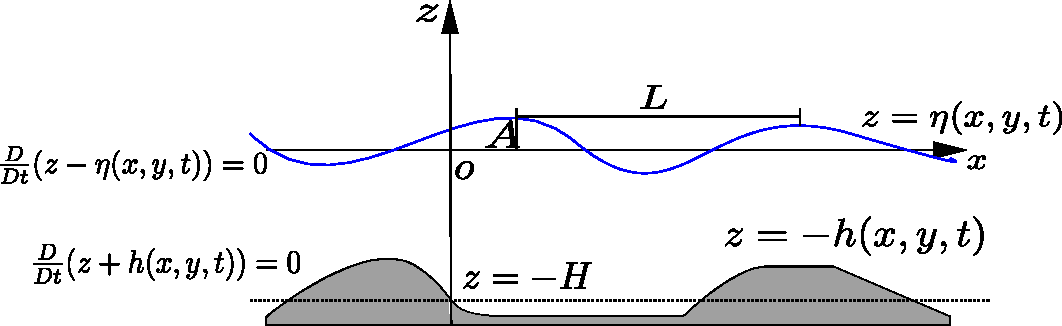
\includegraphics[width=\largefig]{chapters/lopes/pdf/graph.pdf}
\end{center}
\caption{Cross-section of the water wave domain.}
\label{fig:lopes:schematic}
\end{figure}

From the irrotational assumption (see
~\eqref{eq:lopes:euler-b}), we can introduce a velocity
potential function, $\phi(x,y,z,t)$\index{potential} to
obtain Bernoulli's equation:
\begin{equation}\label{eq:lopes:bern}
\frac{\partial \phi}{\partial t}+\frac{1}{2}\nabla \phi \cdot\nabla \phi
+\frac{P}{\rho} +g\, z=f(t),
\end{equation}
where $u=\nabla\phi(x,y,z,t)$ and $f(t)$ stands for an
arbitrary function of integration.  Note that we can remove
$f(t)$ from equation~\eqref{eq:lopes:bern} if $\phi$ is
redefined by $\phi+\int f(t) \dt$.  From the
incompressibility condition (see~\eqref{eq:lopes:euler-c})
the velocity potential satisfies Laplace's equation:
\begin{equation}\label{eq:lopes:lap}
\nabla^2\phi+\frac{\partial^2\phi}{\partial z^2}=0,
\end{equation}
where, from now on, $\nabla$ denotes the horizontal gradient
operator given by
$\nabla=\left(\frac{\partial }{\partial x},\frac{\partial
}{\partial y}\right)\!\!.$ To close
this problem, the following boundary conditions must be
satisfied:
\begin{enumerate}
\item[{\it i})] the kinematic boundary condition for the
  free water surface:
\begin{equation}
\frac{\partial \phi}{\partial
  z}=\frac{\partial\eta}{\partial t}+\nabla\phi\cdot\nabla\eta,\quad
z=\eta;
\end{equation}
\item[{\it ii})] the kinematic boundary condition for the
  impermeable sea bottom:
\begin{equation}
\frac{\partial \phi}{\partial z}+(\nabla\phi\cdot\nabla
h)=-\frac{\partial h}{\partial t}, \quad
z=-h ;
\end{equation}
\item[{\it iii})] the dynamic boundary condition for the
  free water surface:
\begin{equation}\label{eq:lopes:dyn}
\frac{\partial \phi}{\partial t}+ g\eta+\frac{1}{2} \left(|\nabla\phi|^2
+\left(\frac{\partial \phi}{\partial z}\right)^2\right)+ D(\phi)-W(\eta) = 0,
\quad z =\eta,
\end{equation}
\end{enumerate}
where $D(\phi)$ is a dissipative term (see, e.g., the work
by~\cite{DutykhDias2007}).  We assume that this dissipative
term is of the following form:
\begin{equation}\label{eq:lopes:diss}
 D(\phi)=\nu\frac{\partial ^2\phi}{\partial z^2},
\end{equation}
with $\nu=\bar{\mu}/\rho$ and $\bar{\mu}$ an eddy-viscosity
coefficient.  Note that a non-dissipative model means that
there is no energy loss.  This is not acceptable from a
physical point of view, since any real flow is accompanied
by energy dissipation.

In equation~\eqref{eq:lopes:dyn}, $W(\eta)$ is the surface
tension term given by:
\begin{equation}\label{eq:lopes:tension}
 \displaystyle W(\eta)=T\frac{\displaystyle
   \left(1+\left(\frac{\partial \eta}{\partial y}\right)^2\right)\frac{\partial ^2\eta}{\partial x^2}+
   \left(1+\left(\frac{\partial \eta}{\partial x}\right)^2\right)\frac{\partial ^2\eta}{\partial y^2}
   -2\frac{\partial \eta}{\partial x}\frac{\partial
     \eta}{\partial y}\frac{\partial ^2\eta}{\partial  x\partial y}}{(1+|\nabla\eta|^2)^{3/2}},
\end{equation}
where $T$ is the surface tension coefficient.

Using Laplace's equation (see~\eqref{eq:lopes:lap}) it
is possible to rewrite~\eqref{eq:lopes:diss} as
$D(\phi)=-\nu\nabla^2\phi$.  Throughout the literature,
analogous terms were added to the kinematic and dynamic
conditions to absorb the wave energy near the boundaries.
These terms are related with the sponge or damping layers
and, as we will see later, they can be used to modify the
dispersion relations.  In addition, the linearization of
equation~\eqref{eq:lopes:tension} results in
$W(\eta)=T\nabla^2\eta$.  The surface tension effects are
important if short waves are considered.  Although the long
wave assumption is made to derive these extended models,
waves of short length are generated in the domain due to the
waves interaction.  Thus, the inclusion of surface tension
in the small amplitude long wave models may be relevant.  On
the other hand, it is worth to mention that one of the main
goals of the scientific research on Boussinesq wave models
is the improvement of the range of applicability in terms of
the water-depth/wave-length relationship.  We refer the
works by~\cite{WangWuChengEtAl2008} as well
as~\cite{DashDaripa2002}, which included surface tension
effects in the KdV (Korteweg-de Vries) and Boussinesq
equations.

A more detailed description of the above equations is found
in the reference book on waves by~\cite{Whitham1974}, or in
the more recent book by~\cite{Johnson1997}.
%}}}

%{{{ Standard models
\subsection{Standard models}
In this subsection, we present a generic Boussinesq system
using the velocity potential formulation.  To transform
equations~\eqref{eq:lopes:bern}--~\eqref{eq:lopes:tension}
in a dimensionless form, the following scales are
introduced:
\begin{equation}
( x', y')=\frac{1}{L}(x,y),\quad z'=\frac{z}{H}, \quad
  t'=\frac{t\sqrt{gH}}{L},\quad \eta'=\frac{\eta}{A},\quad
  \phi'= \frac{H\phi}{AL\sqrt{gH}},\quad h'=\frac{h}{H},
\end{equation}
together with the small parameters
\begin{equation}
\mu=\frac{H}{L},\quad \varepsilon=\frac{A}{H}.
\end{equation}
In the last equation, $\mu$ is called the long wave
parameter and $\varepsilon$ the small amplitude wave
parameter.  Note that $\varepsilon$ is related with the
nonlinear terms and $\mu$ with the dispersive terms.  For
simplicity, in what follows, we drop the prime notation.

The Boussinesq approach consists in reducing a $3$D problem
to a $2$D one.  This may be accomplished by expanding the
velocity potential in a Taylor power series in terms of $z$.
Using Laplace's equation, in a dimensionless form, we can
obtain the following expression for the velocity potential:
\begin{equation}
\phi(x,y,z,t)=\sum_{n=0}^{+\infty}\left((-1)^n\frac{z^{2n}}{(2n)!}\mu^{2n}\nabla^{2n}\phi_0(x,y,t)+
(-1)^n
\frac{z^{2n+1}}{(2n+1)!}\mu^{2n}\nabla^{2n}\phi_1(x,y,t)\right),
\end{equation}
with
\begin{equation}
\phi_0=\phi\mid_{ z=0},\quad
\phi_1=\left(\frac{\partial \phi}{\partial z}\right)\mid_{z=0}\!.
\end{equation}
From asymptotic expansions, successive approximation
techniques and the kinematic boundary condition for the sea
bottom, it is possible to write $\phi_1$ in terms of
$\phi_0$ (cf.~\cite{ChenLiu1994},~\cite{ZhaoTengCheng2004}).
In this work, without loss of generality, we assume that the
dispersive and nonlinear terms are related by the following
equation:
\begin{equation}\label{eq:lopes:ursell}
\frac{\varepsilon}{\mu^2}=O(1)\ {\rm with}\ \mu<1\ {\rm
  and}\ \varepsilon<1.
\end{equation}
Note that the Ursell number is defined by $\displaystyle
U_r=\frac{\varepsilon}{\mu^2}$ and plays a central role in
deciding the choice of approximations which correspond to
very different physics.  The regime of weakly nonlinear,
small amplitude and moderately long waves in shallow water
is characterized by \eqref{eq:lopes:ursell}
$\left(O(\mu^2)=O(\varepsilon), {\ \rm i.e.,\ }
\frac{H^2}{L^2}\approx\frac{A}{H} \right)$.  Boussinesq
equations account for the effects of nonlinearity
$\varepsilon$ and dispersion $\mu^2$ to the leading order.
When $\varepsilon\gg \mu^2$ , they reduce to the Airy
equations.  When $\varepsilon\ll \mu^2$ they reduce to the
linearized approximation with weak dispersion.  Finally, if
we assume that $\varepsilon\rightarrow 0$ and
$\mu^2\rightarrow 0$, the classical linearized wave equation
is obtained.

A sixth-order spatial derivative model is obtained if
$\phi_1$ is expanded in terms of $\phi_0$ and all terms up
to $O(\mu^8)$ are retained.  Thus, the asymptotic kinematic
and dynamic boundary conditions for the free water surface
are rewritten as follows \footnote{Note that $D$ and $W$
  are, now, dimensionless functions.}:
\begin{subequations}\label{eq:lopes:kindyn}
\begin{align}
&\displaystyle\frac{\partial \eta}{\partial t}+\varepsilon\nabla\cdot(\eta\nabla\phi_0)-\frac{1}{\mu^2}\phi_1+
  \frac{\varepsilon^2}{2}\nabla\cdot(\eta^2\nabla\phi_1)=O(\mu^{6}),
\vspace{0.3cm}\\ &\displaystyle
\frac{\partial \phi_0}{\partial t}+\varepsilon\eta\frac{\partial \phi_1}{\partial t}+\eta +
\frac{\varepsilon}{2}
\left|\nabla\phi_0\right|^2+\varepsilon^2\nabla\phi_0\cdot\eta\nabla\phi_1-\nonumber
\\ & \displaystyle \qquad
-\varepsilon^2\eta\nabla^2\phi_0\phi_1
+\frac{\varepsilon}{2\mu^2}\phi_1^2
+D(\phi_0,\phi_1)-W(\eta) =O(\mu^{6}),
\end{align}
\end{subequations}
where $\phi_1$ is given by:
\begin{multline}\label{eq:lopes:phi_1}
\phi_1= -\mu^{2}\nabla\cdot\left(h\nabla\phi_0\right)
+\frac{\mu^{4}}{6}\nabla\cdot\left(h^3\nabla^3\phi_0\right)
-\frac{\mu^{4}}{2}\nabla\cdot\left(h^2
\nabla^2\cdot\left(h\nabla\phi_0\right)
\right)-\\ -\frac{\mu^6}{120}\nabla\cdot\left(h^5\nabla^5\phi_0\right)+
\frac{\mu^6}{24}\nabla\cdot\left(h^4\nabla^4\cdot\left(h\nabla\phi_0\right)\right)+\frac{\mu^6}{12}\nabla\cdot\left(h^2\nabla^2\cdot\left(h^3\nabla^3\phi_0\right)\right)-\\ -\frac{\mu^6}{4}\nabla\cdot\left(h^2\nabla^2\cdot\left(h^2\nabla^2\cdot\left(h\nabla\phi_0\right)\right)\right)
-\frac{\mu^2}{\varepsilon}\frac{\partial h}{\partial t}-
\frac{\mu^2}{\varepsilon}\frac{\mu^2}{2}\nabla\cdot\left(h^2\nabla\frac{\partial h}{\partial t}\right)+\\ +\frac{\mu^2}{\varepsilon}\frac{\mu^4}{24}\nabla\cdot\left(h^4\nabla^3
\frac{\partial h}{\partial t}\right)
-\frac{\mu^2}{\varepsilon}\frac{\mu^4}{4}\nabla\cdot\left(h^2\nabla^2\left(h^2\nabla\frac{\partial h}{\partial t}\right)\right)+O(\mu^{8}).
\end{multline}
To obtain equation~\eqref{eq:lopes:phi_1}, we assume that
$\displaystyle\frac{\partial h}{\partial t}=O(\varepsilon)$
(cf.~\cite{DutykhDias2007}).
%}}}

%{{{ $2^{nd}$-order model
\subsection{Second-order spatial derivative model}
The  second-order  spatial derivative equations
 are obtained, essentially, via the
slowly varying bottom assumption. In particular, only
$O(h,\nabla h)$ terms are retained.  Also, only $O(\varepsilon)$
nonlinear terms are admitted.  In fact,
the extended ZTC model is written retaining only
$O(\varepsilon,\mu^4)$ terms.

Under these conditions,~\eqref{eq:lopes:kindyn} and
~\eqref{eq:lopes:phi_1} lead to:
\begin{subequations}\label{eq:lopes:kindyn2}
\begin{align}
&\displaystyle\frac{\partial \eta}{\partial t}+\varepsilon\nabla\cdot(\eta\nabla\phi_0)
-\frac{1}{\mu^2}\phi_1=O(\mu^{6}),\vspace{0.3cm}\label{eq:lopes:kindyn2-a}
\\
&\displaystyle\frac{\partial \phi_0}{\partial t}+\eta + \frac{\varepsilon}{2}
\left|\nabla\phi_0\right|^2-\nu^*\varepsilon\nabla^2\phi_0-T^*\mu^2\nabla^2\eta
=O(\mu^{6}),\label{eq:lopes:kindyn2-b}
\end{align}
\end{subequations}
where $\nu^*=\nu\sqrt{H}/(AL\sqrt{g})$, $T^*= T/(gH^2)$ and
\begin{multline}\label{eq:lopes:phi_2}
\phi_1= -\mu^{2}\nabla\cdot\left(h\nabla\phi_0\right)
+\frac{\mu^{4}}{6}\nabla\cdot\left(h^3\nabla^3\phi_0\right)
-\frac{\mu^{4}}{2}\nabla\cdot\left(h^2
\nabla^2\cdot\left(h\nabla\phi_0\right)
\right)-\\ -\frac{2\mu^6}{15}h^5\nabla^6\phi_0-2\mu^6h^4\nabla
h\cdot\nabla^5\phi_0
-\frac{\mu^2}{\varepsilon}\frac{\partial h}{\partial t}+O(\mu^{8}).
\end{multline}
Thus, these extended equations, in terms of the dimensional
variables, are written as follows:
\begin{subequations}\label{eq:lopes:ztc}
\begin{align}
&\frac{\partial\eta}{\partial t}
  +\nabla\cdot[(h+\eta)\nabla{\Phi}] -\frac{1}{2}\nabla\cdot
  [h^{2}\nabla\frac{\partial \eta} {\partial t}]
  +\frac{1}{6}h^{2}\nabla^2\frac{\partial\eta}{\partial t}
  -\frac{1}{15}\nabla\cdot[h\nabla(h\frac{\partial\eta}
    {\partial
      t})]=-\frac{\partial h}{\partial t}, \label{eq:lopes:ztc-a}\\ &\frac{\partial
    \Phi}{\partial t} +\frac{1}{2}|\nabla\Phi|^2+g\eta-
  \frac{1}{15}gh\nabla\cdot(h\nabla\eta)-\nu\nabla^2\Phi-T\nabla^2\eta=0, \label{eq:lopes:ztc-b}
\end{align}
\end{subequations}
where $\Phi$ is the transformed velocity potential given by:
\begin{equation}\label{eq:lopes:phitrans}
\Phi=\phi_0+\frac{h}{15}\nabla\cdot(h\nabla\phi_0) .
\end{equation}
 In this context, the use of the transformed velocity
 potential has two main advantages
 (cf.~\cite{ZhaoTengCheng2004}):
\begin{itemize}
\item[{\it i})] the spatial derivative order is reduced to 2;
\item[{\it ii})] linear dispersion characteristics,
  analogous to the  BEP model proposed
  by~\cite{ChenLiu1994} and the  BEV model
  developed by~\cite{Nwogu1993}, are obtained.
The latter models contain fourth and third-order spatial
derivatives, respectively.
\end{itemize}
%}}}

%{{{ Linear dispersion relation
\section{Linear dispersion relation}\label{sec:lopes:dispersionproperties}
One of the most important properties of a water wave model
is described by the linear dispersion relation.  From this
relation we can deduce the phase velocity, group velocity
and the linear shoaling.

The dispersion relation \index{dispersion relation} of a
linearized water wave model should be in good agreement with
the one provided by the linear wave theory of Airy.


In this section we follow the work by~\cite{DutykhDias2007}.
Moreover, we only present a generalized version of the
dispersion relation for the extended ZTC model with the
dissipative term mentioned above.  We can also include other
damping terms, which are usually used in the sponge layers.

For simplicity, a one horizontal dimensional model is considered.  To
obtain the dispersion relation, a standard test wave is
assumed:
\begin{subequations}\label{eq:lopes:linwave}
\begin{align}
&\eta(x,t)=a\,e^{i(kx-\omega
  t)},\vspace{0.3cm}\\
&\Phi(x,t)=-b\,i\,e^{i(kx-\omega t)},
\end{align}
\end{subequations}
where $a$ is the wave amplitude, $b$ the potential
magnitude, $k=2\pi/L$ the wave number and $\omega$ the
angular frequency.  This wave, described by
equations~\eqref{eq:lopes:linwave}, is the solution of the
linearized extended ZTC model, with a constant depth bottom and an
extra dissipative term, if the following equation is
satisfied:
\begin{equation}\label{eq:lopes:dissdisp}
\omega^2-ghk^2\frac{1+\frac{1}{15}(kh)^2}{1+\frac{2}{5}(kh)^2}+i\nu\omega
k^2=0.
\end{equation}
The dispersion relation given by the last equation is
accurate up to $O((kh)^4)$ or $O(\mu^4)$ when compared with
the Pad\'{e} approximant of order $[2/2]$ of the following
equation:
\begin{equation}\label{eq:lopes:linairy}
\omega^2-ghk^2\frac{\tanh(kh)}{kh}+i\nu\omega k^2=0.
\end{equation}
In fact, equation~\eqref{eq:lopes:linairy} is the dispersion
relation of the full linear problem.

From~\eqref{eq:lopes:dissdisp}, the phase velocity,
$\displaystyle C=\frac{w}{k}$, for this dissipative and extended
ZTC model is given by:
\begin{equation}\label{eq:lopes:phasevel}
C=-\frac{i\nu k}{2}\pm\sqrt{-\left(\frac{\nu
    k}{2}\right)^2+gh\frac{(1+\frac{1}{15}(kh)^2)}{(1+\frac{2}{5}(kh)^2)}}.
\end{equation}
In Fig.~\ref{fig:lopes:dispersion}, we can see the positive
real part of $\displaystyle\left(C/\sqrt{gh}\right)$ as a
function of $kh$ for the following models: full linear
theory (FL), Zhao et al. (ZTC), full linear theory with a
dissipative model (FL\_D) and the improved ZTC model with
the dissipative term (ZTC\_D).
\begin{figure}
\begin{center}
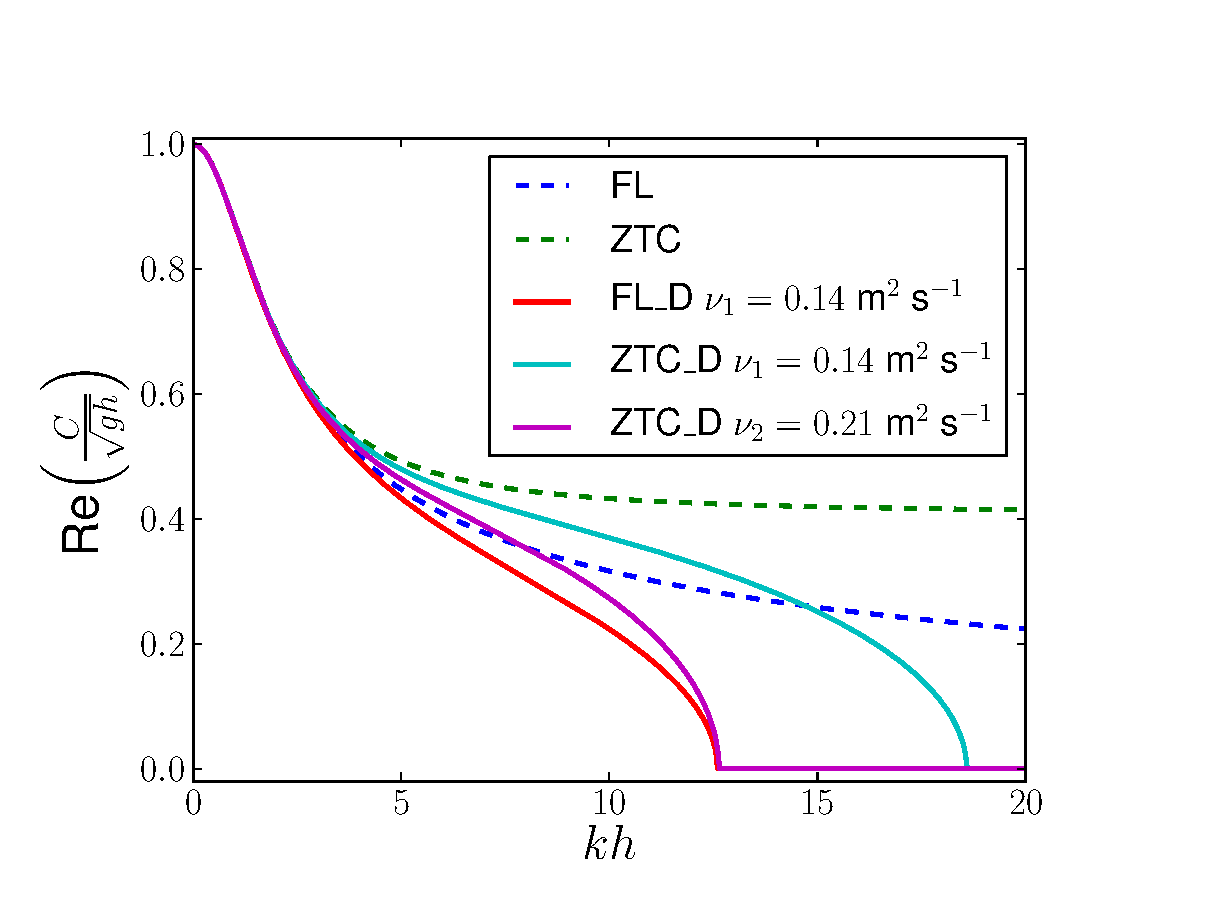
\includegraphics[width=\largefig]{chapters/lopes/pdf/phase_velocity_simple.pdf}
\end{center}
\caption{Positive part of $\displaystyle
  Re\left(C/\sqrt{gh}\right)$ as a function of $kh$ for
  several models.}
\label{fig:lopes:dispersion}
\end{figure}

\noindent From Fig.~\ref{fig:lopes:dispersion}, we can also see that
these two dissipative models admit critical wave numbers
$k_1$ and $k_2$, such that the positive part of
$\displaystyle Re\left(C/\sqrt{gh}\right)$ is zero for
$k\geq k_1$ and $k\geq k_2$, respectively.
We can optimize the value of $\nu$ in the ZTC\_D model in
order to have $k_1=k_2$.
From \eqref{eq:lopes:linairy},  $\displaystyle
Re\left(C/\sqrt{gh}\right)$ is zero for
\begin{equation}
k_1^3=4g\frac{\tanh{(k_1h)}}{\nu^2}.
\end{equation}
Thus, we can obtain the values of $k_1$, in the FL\_D model,
for which short waves no longer propagate for fixed $h$ and
$\nu=\nu_1$ values.  Considering now the real part of
\eqref{eq:lopes:phasevel} equal to zero, we have
\begin{equation}\label{eq:lopes:nu1}
\nu^2=4\frac{gh}{k^2}\left(\frac{1+\frac{1}{15}(kh)^2}{1+\frac{2}{5}(kh)^2}\right).
\end{equation}
Therefore, inserting the previous value of $k_1$ into
\eqref{eq:lopes:nu1} we obtain the corresponding value of
$\nu=\nu_2$, in the ZTC\_D model, for which the same type of waves
do not propagate.
In Fig.~\ref{fig:lopes:dispersion}, we can
see that if $\nu_1=0.14\, $~m$^2\,$~s$^{-1}$ in
the FL\_D model   and $\nu_2=0.21$
m$^2$ s$^{-1}$ in the ZTC\_D model, $k_1=k_2=12.6$ m$^{-1}$
for $h=1$ m.
In this case the time  decayment of the solutions in
the ZTC\_D model is more accentuated than in the FL\_D
model.
Numerical instabilities generated by short length waves can
be eliminated optimizing the viscosity values as shown above.

In general, to improve the dispersion relation we can also
use other transformations like~\eqref{eq:lopes:phitrans}, or
evaluate the velocity potential at $z=-\sigma h$
($\sigma\in[0,1]$) instead of $z=0$
(cf.~\cite{BinghamMadsenFuhrman2008}, \cite{MadsenAgnon2003}
and~\cite{MadsenBinghamSchaffer2003}).
%}}}

%{{{ Wave generation
\section{Wave generation}\label{sec:lopes:wavegeneration}
In this section some of the physical mechanisms responsible
for inducing surface water waves are presented.  We note
that the moving bottom approach is useful for wave
generation due to seismic activities. However, some physical
applications are associated with other wave generation
mechanisms.  For simplicity, we only consider mechanisms to
generate surface water waves along the $x$ direction.

\subsection{Initial conditions}
The simplest way of inducing a wave into a certain domain is
to consider an appropriate initial condition. A useful and
typical case is to assume a solitary wave given by:
\begin{equation}\label{eq:lopes:solita}
\eta(x,t)=a_1\,{\rm sech}^2(kx -\omega t)+a_2\,{\rm
  sech}^4(kx-\omega t)\quad {\rm at\,\,} t=0\,{\tt s},
\end{equation}
\begin{equation}\label{eq:lopes:solitb}
u(x,t)=a_3\,{\rm sech}^2(k x-\omega t) \quad {\rm at\,\,}
t=0\,{\tt s},
\end{equation}
where the parameters $a_1$ and $a_2$ are the wave amplitudes
and $a_3$ is the magnitude of the velocity in the $x$
direction.  Since we use a potential formulation, $\Phi$ is
given by:
\begin{equation}\label{eq:lopes:solitp}
\Phi(x,t)=-\frac{2a_3\,e^{2\omega t }}{k\,(e^{2\omega t
  }+e^{2k x})}+ K_1(t) \quad {\rm at\,\,} t=0\,{\tt s},
\end{equation}
where $K_1(t)$ is a time-dependent function of integration.

We remark that the above solitary wave given by
~\eqref{eq:lopes:solita} and~\eqref{eq:lopes:solitb}, but
for all time $t$, was presented as a solution of the
extended Nwogu's Boussinesq model in~\cite{Walkley1999}
and~\cite{WeiKirby1995} .

\subsection{Incident wave}
For time-dependent wave generation, it is possible to
consider waves induced by a boundary condition.  This
requires that the wave surface elevation and the velocity
potential must satisfy appropriate boundary conditions,
e.g., Dirichlet or Neumann conditions.\index{boundary
  conditions}

The simplest case is to consider a periodic wave given by:
\begin{equation}\label{eq:lopes:dirichleteta}
\eta(x,t)=a \sin(kx-\omega t)
\end{equation}
\begin{equation}\label{eq:lopes:dirichletphi}
\Phi(x,t)=-\frac{c}{k}\cos(k x-\omega t)+K_2(t),
\end{equation}
where $c$ is the wave velocity magnitude and $K_2(t)$ is a
time-dependent function of integration.  This function
$K_2(t)$ must satisfy the initial condition of the problem.
Note that the parameters $a,c,k$ and $\omega$ are not
arbitrary, but confined to values consistent with the
dispersion equation~\eqref{eq:lopes:dissdisp}.  We can also
consider the superposition of water waves as solutions of
the full linear problem with a constant depth.
%}}}

%{{{ Source function
\subsection{Source function}
In the work by~\cite{WeiKirbySinha1999}, a source
function\index{source function} for the generation of
surface water waves was derived.  This source function was
obtained, using Fourier transform and Green's functions, to
solve the linearized and nonhomogeneous equations of
the~\cite{Peregrine1967} and~\cite{Nwogu1993} models.  This
mathematical procedure can also be adapted here to deduce
the source function.

We consider a monochromatic Gaussian wave generated by the
following source function:
\begin{equation}\label{eq:lopes:src}
S(x,t)=D^* \exp(-\beta (x-x_s)^2)\cos(\omega t),
\end{equation}
with $D^*$ given by:
\begin{equation}
\displaystyle
D^*=\frac{\sqrt{\beta}}{\omega\sqrt{\pi}}a\exp(\frac{k^2}{4\beta})\frac{2}{15}h^3k^3g.
\end{equation}
In the above expressions $x_s$ is the center line of the
source function and $\beta$ is a parameter associated with
the width of the generation band
(cf.~\cite{WeiKirbySinha1999}).  Note that $S(x,t)$ should
be added to the right-hand side of
equation~\eqref{eq:lopes:ztc-a}.
%}}}

%{{{ Reflective walls and sponge layers
\section{Reflective walls and sponge layers}\label{sec:lopes:boundaryconditions}

Besides the incident wave boundaries where the wave profiles
are given, we must close the system with appropriate
boundary conditions.  We consider two more types of
boundaries:
\begin{itemize}
\item[{\it i})] full reflective boundaries;\index{reflective
  boundaries}
\item[{\it ii})] sponge layers.
\end{itemize}
The first case is modelled by the following equations:
\begin{equation}\label{eq:lopes:fullrefl}
\frac{\partial \Phi}{\partial n}=0\quad {\rm
  and}\quad\frac{\partial \eta}{\partial n}=0\quad {\rm
  on\,\, } \Gamma,
\end{equation}
where $n$ is the outward unit vector normal to the boundary
$\Gamma$ of the domain $\Omega$.

Regarding the second case, we consider equations
~\eqref{eq:lopes:fullrefl} and an extra artificial term,
often called sponge \index{sponge-layers} or damping layer,
given by $\nu\nabla^2\Phi$ (see equation
~\eqref{eq:lopes:ztc-b}), acting in a neighborhood of the
boundary $\Gamma$.  In this way, the reflected energy can be
controlled. Moreover, we can prevent unwanted wave
reflections and avoid complex wave interactions.  It is also
possible to simulate effects like energy dissipation by wave
breaking.

In fact, a sponge layer is a subset $\Omega_S$ of $\Omega$
where some extra viscosity term is added.  As mentioned
above, the system of equations can incorporate several extra
damping terms, like that one provided by the inclusion of a
dissipative model. Thus, the viscosity coefficient $\nu$ can
be described by a function of the following form:
\begin{equation}\label{eq:lopes:sponge}
\nu(x,y)= \left\{
\begin{matrix}
0,& (x,y)\not\in\Omega_S ,\vspace{0.3cm}\\ \displaystyle
n_1\frac{\displaystyle\exp{\left(\frac{d_{\Omega_S}-d(x,y)}
    {d_{\Omega_S}}\right)^{n_2}}-1}{\exp(1)-1},& (x,y)
\in\Omega_S,
\end{matrix}
\right.
\end{equation}
where $n_1$ and $n_2$ are, in general, experimental
parameters, $d_{\Omega_S}$ is the sponge-layer diameter and
$d(x,y)$ stands for a distance function between a point
$(x,y)$ and the intersection of $\Gamma$ with the boundary
of $\Omega_S$ (see, e.g.,~\cite{Walkley1999}).
%}}}

%{{{ Numerical Methods
\section{Numerical methods}\label{sec:lopes:numericalmethods}
We start this section by noting that a detailed description
of the implemented numerical methods referred bellow can be
found in the work of~\cite{Lopes2007}.

For simplicity, we only consider the system described by
equations~\eqref{eq:lopes:ztc} restricted to a stationary
bottom and without dissipative, surface tension or extra
source terms.

The model variational formulation is written as follows:
\begin{subequations}\label{eq:lopes:varform}
\begin{align}
\begin{split}
&\displaystyle \int_\Omega\frac{\partial \eta}{\partial t}\vartheta_1\, \dx\, \mathrm{d}y
  +\frac{1}{2}\int_\Omega
  h^2\nabla\left(\frac{\partial \eta}{\partial t}\right)\cdot\nabla\vartheta_1\,
  \dx\, \mathrm{d}y- \frac{1}{6}\int_\Omega \nabla\left(
  \frac{\partial \eta}{\partial t}\right)\cdot\nabla(h^2\vartheta_1)\,
  \dx\, \mathrm{d}y+\\ &\quad \quad\displaystyle +
  \frac{1}{15}\int_\Omega
  h\nabla\left(h\frac{\partial \eta}{\partial t}\right)\cdot
  \nabla\vartheta_1\, \dx\, \mathrm{d}y- \frac{1}{15}\int_\Gamma
  h\frac{\partial h}{\partial n}\,\frac{\partial \eta}{\partial t}\,\vartheta_1\, \ds=
  \\ &\quad\quad=\displaystyle
  \int_\Omega(h+\eta)\nabla\Phi\cdot\nabla\vartheta_1\,
  \dx\, \mathrm{d}y -\int_\Gamma(h+\eta)\frac{\partial \Phi}{\partial n}\vartheta_1\, \ds
  +\frac{2}{5}\int_\Gamma
  h^2\frac{\partial }{\partial t}\left(\frac{\partial \eta}{\partial n}\right)\vartheta_1 \ds,
\vspace{0.3cm}
\end{split} \\
\begin{split}
&\displaystyle \int_\Omega \frac{\partial \Phi}{\partial t}\,\vartheta_2\,
  \dx\, \mathrm{d}y= -\frac{1}{2}\int_\Omega|\nabla\Phi|^2\vartheta_2\,
  \dx\, \mathrm{d}y -g\int_\Omega \eta\,\vartheta_2\,
  \dx\, \mathrm{d}y-\\ &\qquad\qquad\qquad\displaystyle-\frac{g}{15}\int_\Omega
  h\nabla\eta\cdot\nabla(h\vartheta_2)\, \dx\, \mathrm{d}y
  +\frac{g}{15}\int_\Gamma h^2\frac{\partial \eta}{\partial n}\,\vartheta_2\,
  \ds,
\end{split}
\end{align}
\end{subequations}
where the unknown functions $\eta$ and $\Phi$ are the wave
surface elevation and the transformed velocity potential,
whereas $\vartheta_1$ and $\vartheta_2$ are the test
functions defined in appropriate spaces.

We use a predictor-corrector \index{Predictor--Corrector}
scheme with an initialization provided by an explicit
Runge--Kutta\index{Runge--Kutta} method for the time
integration. In the DOLFWAVE code these routines are
implemented in the PredCorr and RungeKutta classes (see {\tt
  dolfwave/src/predictorcorrector} and {\tt
  dolfwave/src/rungekutta}).

  Note that the discretization of equations
  ~\eqref{eq:lopes:varform} can be written in the following
  form:
\begin{equation}
M\dot U=F(t,U),
\end{equation}
where $\dot U$ and $U$ refer to $\displaystyle
\left(\frac{\partial \eta}{\partial t},\frac{\partial \Phi}{\partial t}\right)$ and
$(\eta,\Phi)$, respectively.  The coefficient matrix $M$ is
given by the left-hand sides of~\eqref{eq:lopes:varform},
whereas the known vector $F$ is related with the right-hand
sides of the same equations.  In this way, the fourth-order
Adams-Bashforth-Moulton method can be written as follows:
\begin{subequations}\label{eq:lopes:pc}
\begin{align}
&\displaystyle MU^{(0)}_{n+1}=MU_n+\frac{\Delta
    t}{24}[55{F}(t_n,U_n)-59{F}(t_{n-1},U_{n-1})+37{F}(t_{n-2},U_{n-2})-9{F}(t_{n-3},U_{n-3})],
\vspace{0.3cm} \label{eq:lopes:pc-a}\\ \displaystyle
&MU^{(1)}_{n+1}=MU_n+\frac{\Delta
  t}{24}[9{F}(t_{n+1},U^{(0)}_{n+1})+19{F}(t_n,U_n)-5{F}(t_{n-1},U_{n-1})+{F}(t_{n-2},U_{n-2})],\label{eq:lopes:pc-b}
\end{align}
\end{subequations}
where $\Delta t$ is the time step, $t_n=n\Delta t$ $(n\in
\mathbb{N})$ and $U_n$ is $U$ evaluated at $t_n$.  The
predicted and corrected values of $U_n$ are denoted by
$U_n^{(0)}$ and $U_n^{(1)}$, respectively.  The
corrector-step equation~\eqref{eq:lopes:pc-b} can be
iterated as function of a predefined error between
consecutive time steps.  For more details see,
e.g.,~\cite{HairerWanner1991a} or~\cite{Lambert1991}.

The \ufl form file for the declaration of the spatial
discretization of \eqref{eq:lopes:varform} using Lagrange
$P_1$ elements and including  dissipative and
source terms is presented below (see {\tt
  dolfwave/src/2hdforms/Zhao.ufl}).
\begin{python}
P=FiniteElement("Lagrange",triangle,1) # Linear Lagrange element in triangles
Th=P*P # Product space for basis functions

# eta_t: time derivative of the surface elevation
# phi_t: time derivative of the velocity potential
(eta_t,phi_t)=TrialFunctions(Th)

# p: test function for eta_t
# q: test function for phi_t
(p,q)=TestFunctions(Th)

eta=Coefficient(P) # Surface elevation
phi=Coefficient(P) # Velocity potential

h=Coefficient(P) # Depth function
g=Constant(triangle) # Gravity acceleration

# Several types of sponge layers are considered
sp_eta=Coefficient(P) # Viscous frequency coefficient of eta
sp_lap_eta=Coefficient(P) # Viscosity coefficient of Laplacian of eta
sp_phi=Coefficient(P) # Viscous frequency coefficient of phi
sp_lap_phi=Coefficient(P) # Viscosity coefficient of Laplacian of phi

# Source function for the surface elevation equation
srceta=Coefficient(P)

# Normal Vector for boundary contributions
n=P.cell().n

# Bilinear form declaration for M
# Contribution from the surface elevation equation
a0=eta_t*p*dx
a1=(1./2.)*inner(h*h*grad(eta_t),grad(p))*dx
a2=-(1./6.0)*inner(grad(eta_t),grad(h*h*p))*dx
a3=(1./15.0)*inner(h*grad(h*eta_t),grad(p))*dx
a4=-(1./15.)*h*inner(grad(h),n)*eta_t*p*ds # Boundary contribution

# Contribution from the velocity potential equation
a5=(phi_t*q)*dx

# a: bilinear form
# See 'dolfwave/src/formsfactory/bilinearforminit.cpp'
a=a0+a1+a2+a3+a4+a5

# Linear Variational form declaration for F(t,U)
# Contribution from the surface elevation equation
l0=inner(((h+eta))*grad(phi0),grad(p))*dx

# Contribution from the velocity potential equation
l1=-(1./2.)*inner(grad(phi0),grad(phi0))*q*dx
l2=-g*(eta*q)*dx
l3=-g*(1.0/15.0)*inner(h*grad(eta),grad(h*q))*dx

# Sponge layers contributions
l4=-sp_eta*eta*p*dx-sp_lap_eta*inner(grad(eta),grad(p))*dx
l5=-sp_phi*phi0*q*dx-sp_lap_phi*inner(grad(phi0),grad(q))*dx

# Source function for the surface elevation equation
l6=srceta*p*dx

# L: linear form
# See 'dolfwave/src/formsfactory/linearforminit.cpp'
L=l0+l1+l2+l3+l4+l5+l6
\end{python}
%}}}

%{{{ Numerical Applications
\section{Numerical applications}\label{sec:lopes:numericaltests}
\subsection{Solitary wave over a submerged bar}
In this subsection, we simulate the propagation of a
solitary wave passing through a submerged bar.  We describe
the problem along with the DOLFWAVE code used to solve
it. This C++ code should start with the inclusion of the
DOLFWAVE library.
\begin{c++}
#include <dolfwave.h>
using namespace dolfin::dolfwave;
\end{c++}
The initial condition for the wave surface elevation is
given by~\eqref{eq:lopes:solita} and implemented as follows:
\begin{c++}
class ElevationInit : public Expression
{
  void eval(Array<double> & values,const Array<double> & x) const
  { // Wave parameters (see Walkley [1999])
    double c=sqrt(1.025), H=0.4;
    double ca=-0.4, cb=ca+1.0/3.0;
    double center=-5.0;
    double a1=(H/3.0)*(sqr(c)-1)/(cb-ca*sqr(c));
    double a2=-(H/2.0)*sqr((sqr(c)-1)/c)*(cb+2.0*ca*sqr(c))/(cb-ca*sqr(c));
    double k=(1.0/(2.0*H))*sqrt((sqr(c)-1)/(cb-ca*sqr(c)));
    values[0]=a1/sqr(cosh(k*(x[0]-center)))+a2/sqr(sqr(cosh(k*(x[0]-center))));
  }
};
\end{c++}
Moreover, the initial condition for the velocity potential
is defined by~\eqref{eq:lopes:solitp} and implemented using
the following code:
\begin{c++}
class PotentialInit :  public Expression
{
  void eval(Array<double> & values,const Array<double> & x) const
  { //Wave parameters
    double c=sqrt(1.025), H=0.4;
    double ca=-0.4, cb=ca+1.0/3.0;
    double center=-5.0;
    double a3=sqrt(H*g_e)*(sqr(c)-1)/c;
    double k=(1.0/(2.0*H))*sqrt((sqr(c)-1)/(cb-ca*sqr(c)));
    double cnst=4.0*a3/(2.0*k*(1+exp(2.0*k*(-25.)))); //Constant of integration
    values[0]=-4.0*a3/(2.0*k*(1+exp(2.0*k*(x[0]-center))))+cnst;
  }
};
\end{c++}
The sea bottom $h$ ({\tt m}) is described by the following
continuous and piecewise differentiable function:
\begin{equation}\label{eq:lopes:piecewisebottom}
h(x)=\begin{cases}
0.4& {\rm if}\quad -25 \leq x\leq 6\\
-0.05x+0.7& {\rm if}\quad 6< x\leq 12\\
0.1& {\rm if}\quad 12< x\leq 14\\
0.1x-1.3& {\rm if}\quad 14< x\leq 17\\
0.4& {\rm if}\quad 17< x\leq 25
\end{cases}  ({\tt m})
\end{equation}
which is implemented by:
\begin{c++}
class Depth :  public Expression
{
  void eval(Array<double> & values,const Array<double> & x) const
  {
    double retrn=0.0;
    if(x[0]<=6.0)
      retrn=0.4;
    else if(x[0]<=12.0)
      retrn=-0.05*x[0]+0.7;
    else if(x[0]<=14.0)
      retrn=0.1;
    else if(x[0]<=17.0)
      retrn=0.1*x[0]-1.3;
    else retrn=0.4;
    values[0]=retrn;
  }
};
\end{c++}
The main code starts with the creation of an object of the
Dolfwave class by calling its constructor.  Here, we simulate
the wave propagation during $25$ s using a time step of
$0.001$ s.  The \ufl\ form file used in this problem, which
is identified by ``Zhao\_1D'', corresponds to the one
horizontal dimensional version of~\eqref{eq:lopes:varform}.
We use a LU solver provided by the PETSc algebra backend
(see Chapter~\ref{chap:langtangen}).  Here we use Viper for
previewing the numerical solutions, which are saved in the
``output'' directory using a simple ASCII format denoted by
``xyz''.
\begin{c++}
int main( )
{
  Dolfwave dw(25000 /*Number of steps*/,
              0.001 /*Time step*/,
              "Zhao_1D" /*Variational form identifier*/,
              "LU_P" /*Linear solver type*/,
              "viper" /*Preview program*/,
              "output" /*Output directory*/,
              "xyz" /*File output format*/);
\end{c++}
The spatial domain is the interval $[-25,25]$ ({\tt m})
which is discretized using 201 nodes.
\begin{c++}
  Interval mesh(201,-25,25);
\end{c++}
Now all the known functions are initialized.  Sponge layers
or source functions are not used here.
\begin{c++}
  Depth depth; // Depth function
  ElevationInit eta_init; // Initial condition for the surface elevation
  PotentialInit phi_init;  // Initial condition for the velocity potential
  Constant zero(0.0); // Sponge layers and source function are 0
 \end{c++}
From the bilinear and linear forms of the variational
formulation, all the finite element matrices and vectors are created.
\begin{c++}
  dw.FunctionSpaceInit(mesh); // Initialization of the function spaces
  dw.BilinearFormInit(mesh,depth); // Initialization of the bilinear form 'a'
  dw.MatricesAssemble( ); // Initialization of the system matrices
  dw.FunctionsInit( ); // Initialization of the surface elevation and velocity potential
  dw.LinearFormsInit(depth, zero, zero, zero, zero, zero); // Initialization of the linear form 'L'
  dw.InitialCondition(eta_init,phi_init); // Setting the initial conditions
  dw.VectorInit( ); // Initialization of the auxiliary vectors for the time integration schemes
\end{c++}
We only need to make an initial factorization for the LU
solver, since the system matrix does not depend on time.
\begin{c++}
dw.LUFactorization(true); // Reuse the LU factorization throughout the time integration routines
\end{c++}
The output of the symmetric of the depth function is given
by:
\begin{c++}
  dw.DepthPlot(mesh,depth,true); // Plot the symmetric of the depth function h
\end{c++}
Now, the time integration routines are used.  The
Adams--Bashforth--Moulton method described in
equations~\eqref{eq:lopes:pc} is initialized by a
fourth-order explicit Runge--Kutta scheme.
\begin{c++}
  dw.RKInit("exp4"); // Choose the explicit 4th-order Runge-Kutta for initialization
  dw.RKSolve( ); // Use the Runge-Kutta for the 3 initial steps
  dw.PCInit(mesh,true); // Initialization of the predictor-corrector with multi-step corrector

  // Advance in time with the predictor-corrector scheme
  for(dolfin::uint i=4; i<dw.MaxSteps+1;i++)
    {
      dw.PCSolve( ); // Adams-Bashforth-Moulton method
      if (!(i%100)) // Save and preview the surface elevation with a gap of 100 iterations
      dw.Plot(mesh,true /*eta preview*/, false /*phi preview*/,
                         true /*eta save*/, false /*phi save*/);
    }
  return (EXIT_SUCCESS); // Finish the process
}
\end{c++}
 In this case only the wave surface elevation is saved and
 previewed using the Plot function.  The solution provided
 by this code, for $x\in[-10,25]$ ({\tt m}), is given in
 Fig.~\ref{fig:lopes:submergedbar}.
\begin{figure}
\begin{center}
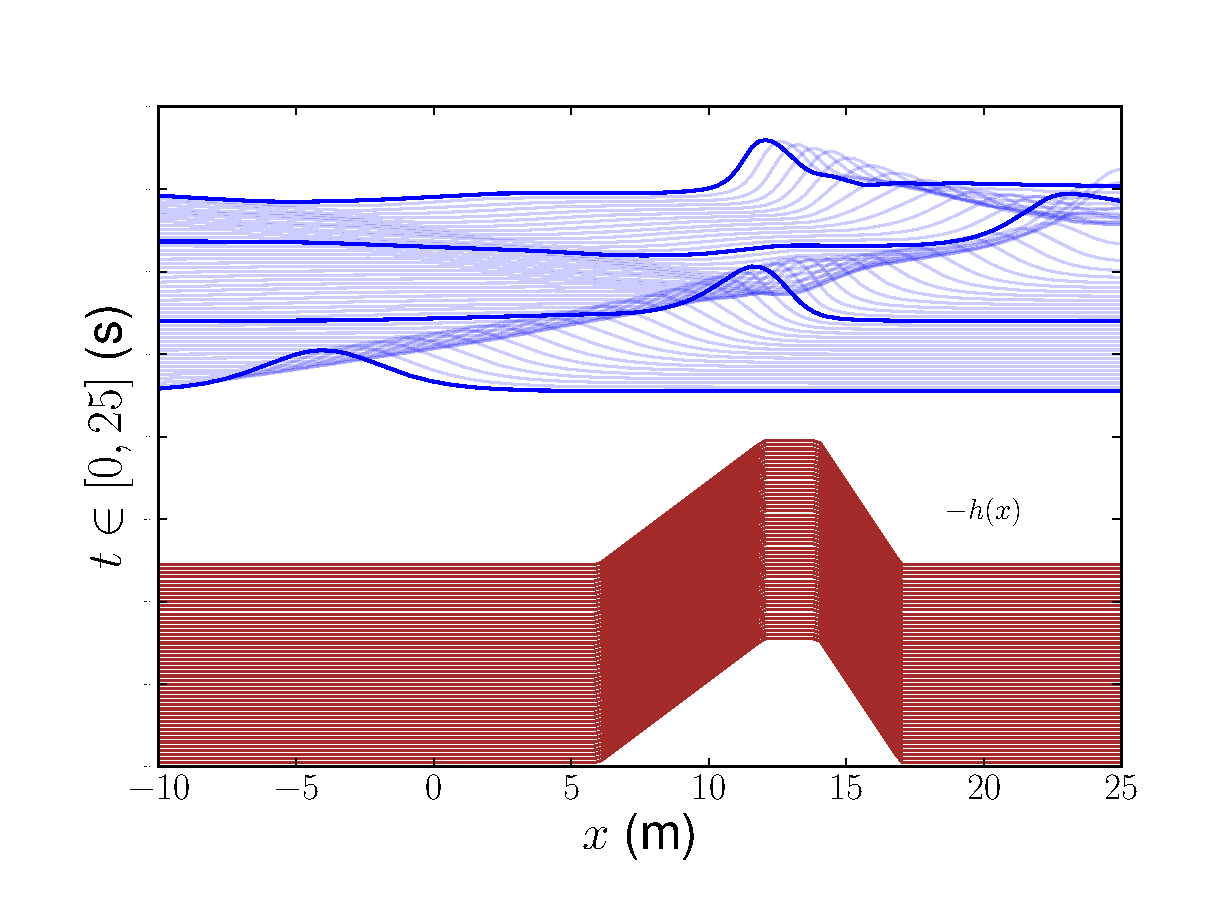
\includegraphics[width=\largefig]{chapters/lopes/pdf/submergedbar.pdf}
\end{center}
\caption{Detailed view of a wave passing through a submerged
  bar}
\label{fig:lopes:submergedbar}
\end{figure}

We remark that the shoaling effect over the submerged bar is
clearly observed, both for the incident and reflected
waves. A good agreement among the solutions presented here
with those provided by other models is achieved (see {\tt
  dolfwave/demo/1HD/submergedbar}).

\subsection{Harbor}
In this subsection, we present some numerical results about
the propagation of surface water waves in a harbor with a
geometry similar to that one of Fig.~\ref{fig:lopes:harbor}.
The finite element discretization of
equations~\eqref{eq:lopes:varform} is declared in the
\ufl\ form file given in
section~\ref{sec:lopes:numericalmethods}.  The DOLFWAVE demo
code for this example is available at {\tt
  dolfwave/demo/2HD/harbor}.

The color scale used in
Figs.~\ref{fig:lopes:harbor_depth}--\ref{fig:lopes:potential1}
is presented in Fig.~\ref{fig:lopes:scale}.  A schematic
description of the fluid domain, namely the bottom profile
and the sponge layer can be seen in
Figs.~\ref{fig:lopes:harbor_depth}
and~\ref{fig:lopes:sponge}, respectively.  Note that a
piecewise linear bathymetry is considered.  Sponge layers of
the type $\nu\nabla^2\Phi$ with the viscosity coefficients
given by equation~\eqref{eq:lopes:sponge} are used to absorb
the wave energy at the outflow region and to avoid strong
interaction between incident and reflected waves in the
harbor entrance.  A monochromatic periodic wave is
introduced at the indicated boundary (Dirichlet BC) in
Fig.~\ref{fig:lopes:sponge}.  This is achieved by
considering waves induced by a periodic Dirichlet boundary
condition, described by the
equations~\eqref{eq:lopes:dirichleteta}
and~\eqref{eq:lopes:dirichletphi}, with the following
characteristics:
\smallskip
\begin{center}
\renewcommand{\arraystretch}{1.3}
\begin{tabular}{|c|c|c|}
\hline $a$ & wave amplitude & $0.25 \,{\tt m}$\\ \hline
$\omega$ & wave angular frequency & $0.64715 \,{\tt
  s}^{-1}$\\ \hline $p$ & wave period & $4.06614 \,{\tt
  s}$\\ \hline $k$ & wave number & $0.06185 \,{\tt
  m}^{-1}$\\ \hline $L$ & wave length & $101.59474 \,{\tt
  m}$\\ \hline $b$ & wave potential magnitude& $3.97151
\,{\tt m}^2{\tt s}^{-1}$\\ \hline $c$ & wave velocity
magnitude& $0.24562 \,{\tt m\, s}^{-1}$ \\ \hline
$\varepsilon$& small amplitude parameter &
$0.01823$\\ \hline $\mu$ & long wave parameter &
$0.13501$\\ \hline
\end{tabular}
\end{center}
\smallskip
Full reflective walls are assumed as boundary conditions in
all domain boundary except in the harbor entrance.  In
Fig.~\ref{fig:lopes:elevation} a snapshot of the wave
surface elevation is shown at the time $t_s=137\,{\tt s}$.

 A zoom of the image, which describes the physical potential
 $\phi_0(x,y)$ and velocity vector field in the still water
 plane, is given in the neighborhood of the point
 $P_3=(255,-75)\,({\tt m})$ at $t_s$ (see
 Fig.~\ref{fig:lopes:potential1}).  The
 Figs.~\ref{fig:lopes:etap} and~\ref{fig:lopes:velp}
 represent the wave surface elevation and water speed as a
 function of the time, at the points $P_1=(-350, 150)\,({\tt
   m}),\, P_2=(-125,60)\,({\tt m})$ and $P_3$.
\begin{figure}
\begin{center}
% Vertical position
%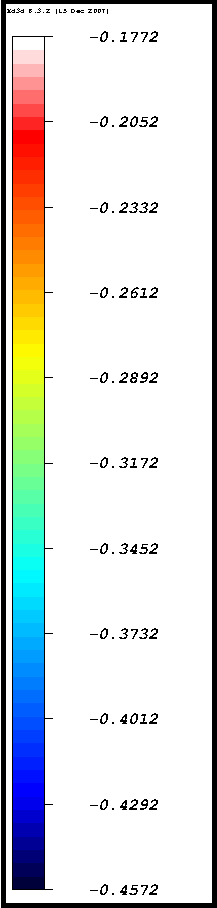
\includegraphics[width=1.0cm]{chapters/lopes/pdf/table.pdf}
% Horizontal position
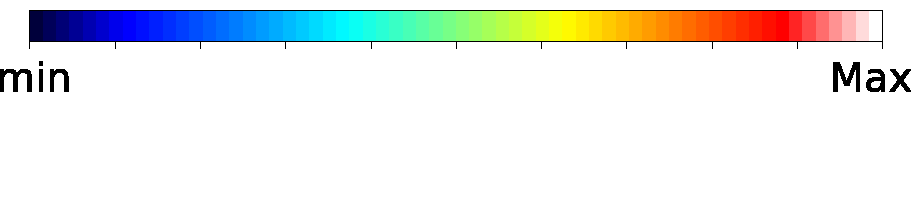
\includegraphics[width=6.0cm]{chapters/lopes/pdf/scale.pdf}
\end{center}
\caption{Color scale.}
\label{fig:lopes:scale}
\end{figure}

\begin{figure}
\begin{center}
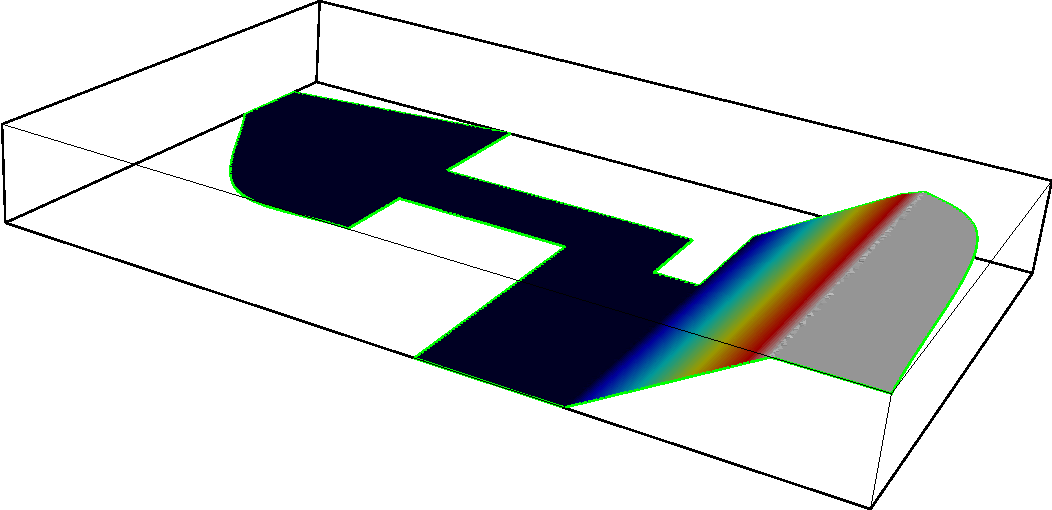
\includegraphics[width=\largefig]{chapters/lopes/pdf/depth.pdf}
\end{center}
\caption{Impermeable bottom $[{\tt Max}=-5.316\,{\tt m},{\tt
      min}=-13.716\,{\tt m}]$.}
\label{fig:lopes:harbor_depth}
\end{figure}
\begin{figure}
\begin{center}
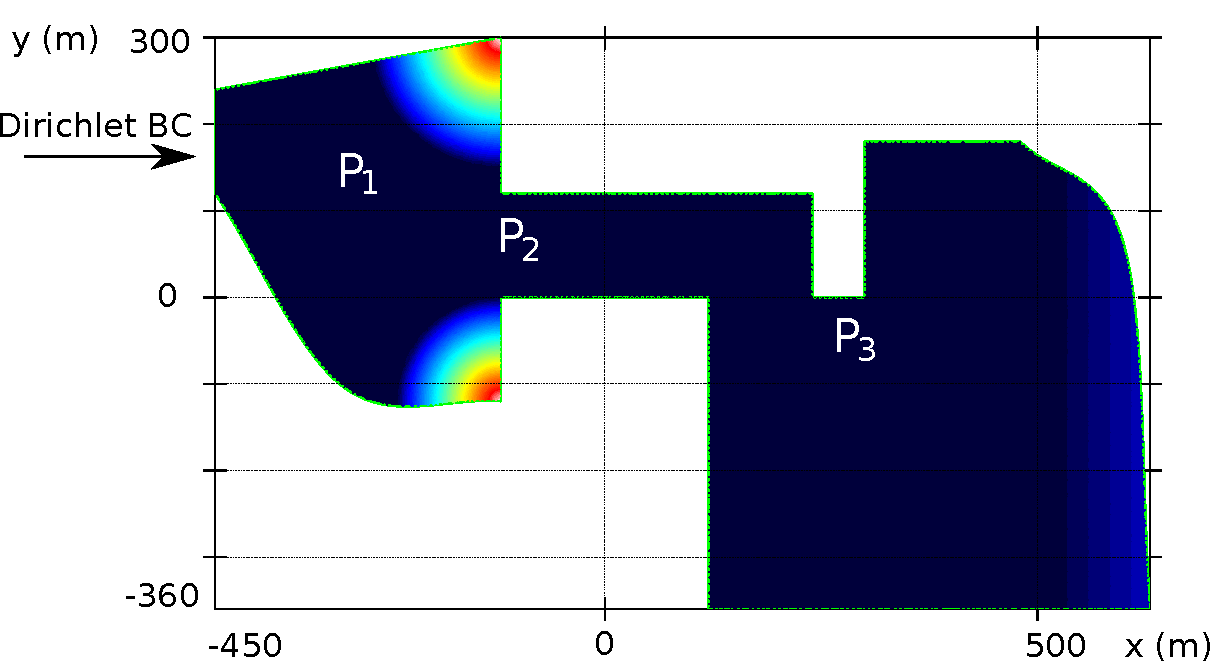
\includegraphics[width=\largefig]{chapters/lopes/pdf/sponge.pdf}
\end{center}
\caption{Sponge layer (viscosity $\nu(x,y)$) $[{\tt Max}
    \approx 0.1\,{\tt m}^2{\tt s}^{-1}, {\tt min}=0 \,{\tt
      m}^2{\tt s}^{-1}]$.}
\label{fig:lopes:sponge}
\end{figure}
\begin{figure}
\begin{center}
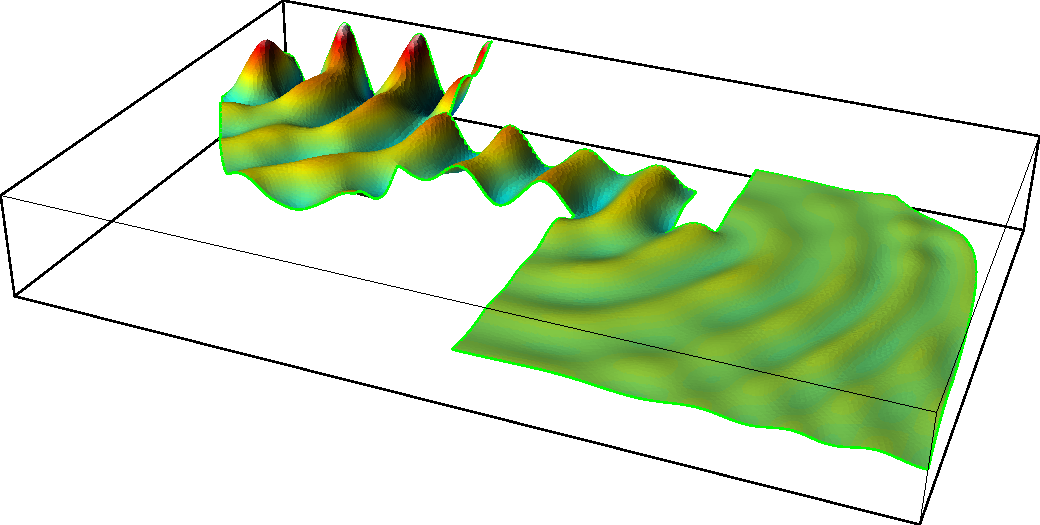
\includegraphics[width=\largefig]{chapters/lopes/pdf/eta.pdf}
\end{center}
\caption{Wave surface elevation $[{\tt Max}\approx 0.63\,{\tt m},
    {\tt min}\approx-0.73\,{\tt m}] $.}
\label{fig:lopes:elevation}
\end{figure}
\begin{figure}
\begin{center}
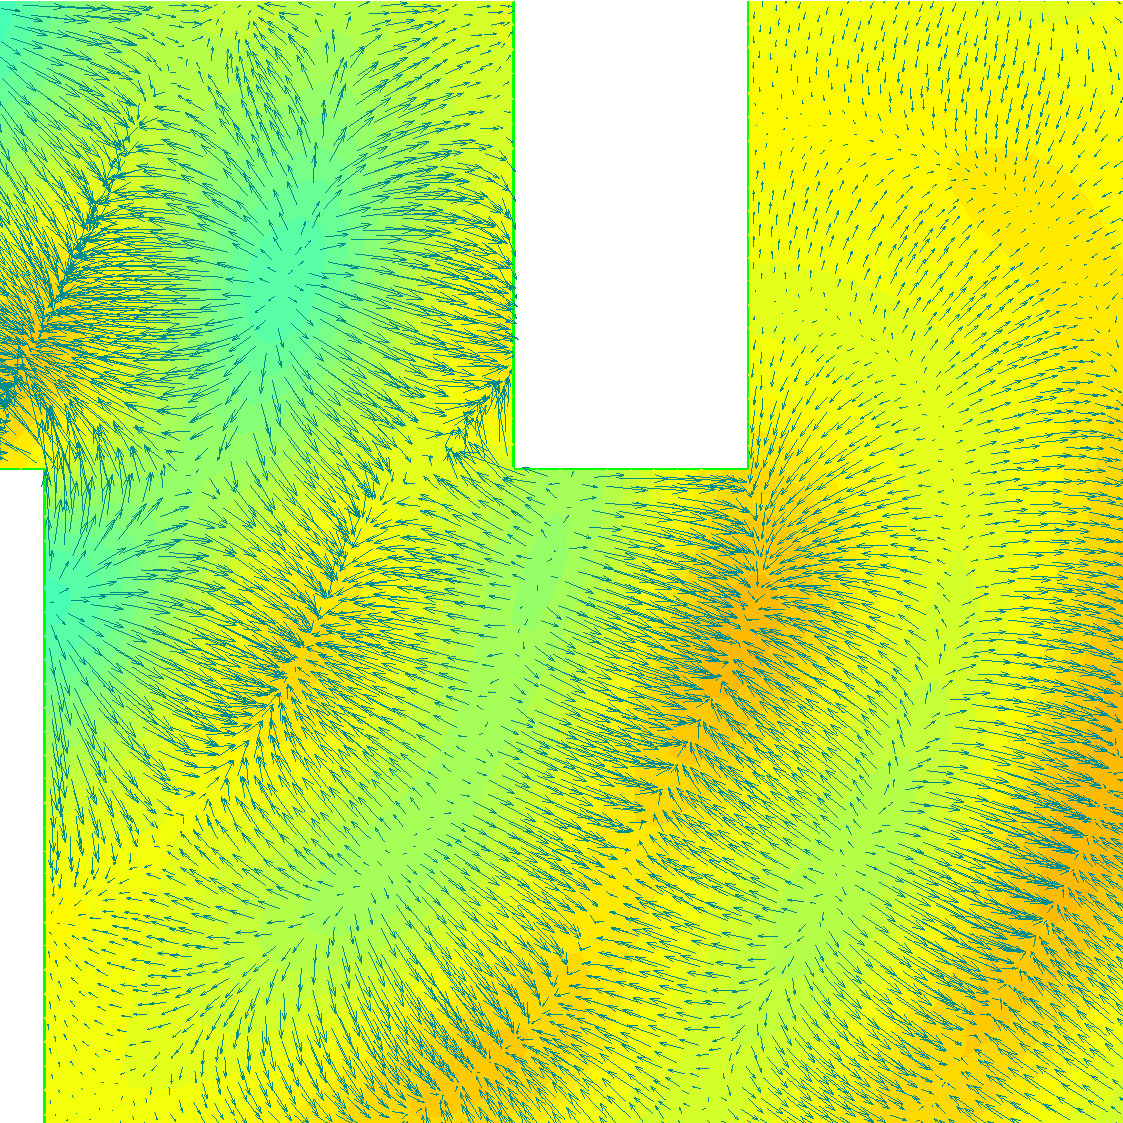
\includegraphics[width=\largefig]{chapters/lopes/pdf/pvel2.pdf}
\end{center}
\caption{Velocity vector field at $z=0$ and potential
  $\phi_0(x,y,t_s)$ near $P_3$. Potential values in
  $\Omega$: $[{\tt Max}\approx 14.2\,{\tt m}^{2}{\tt
      s}^{-1}, {\tt min}\approx-12.8\, {\tt m}^{2}{\tt s}^{-1}]$.}
\label{fig:lopes:potential1}
\end{figure}
\begin{figure}
\begin{center}
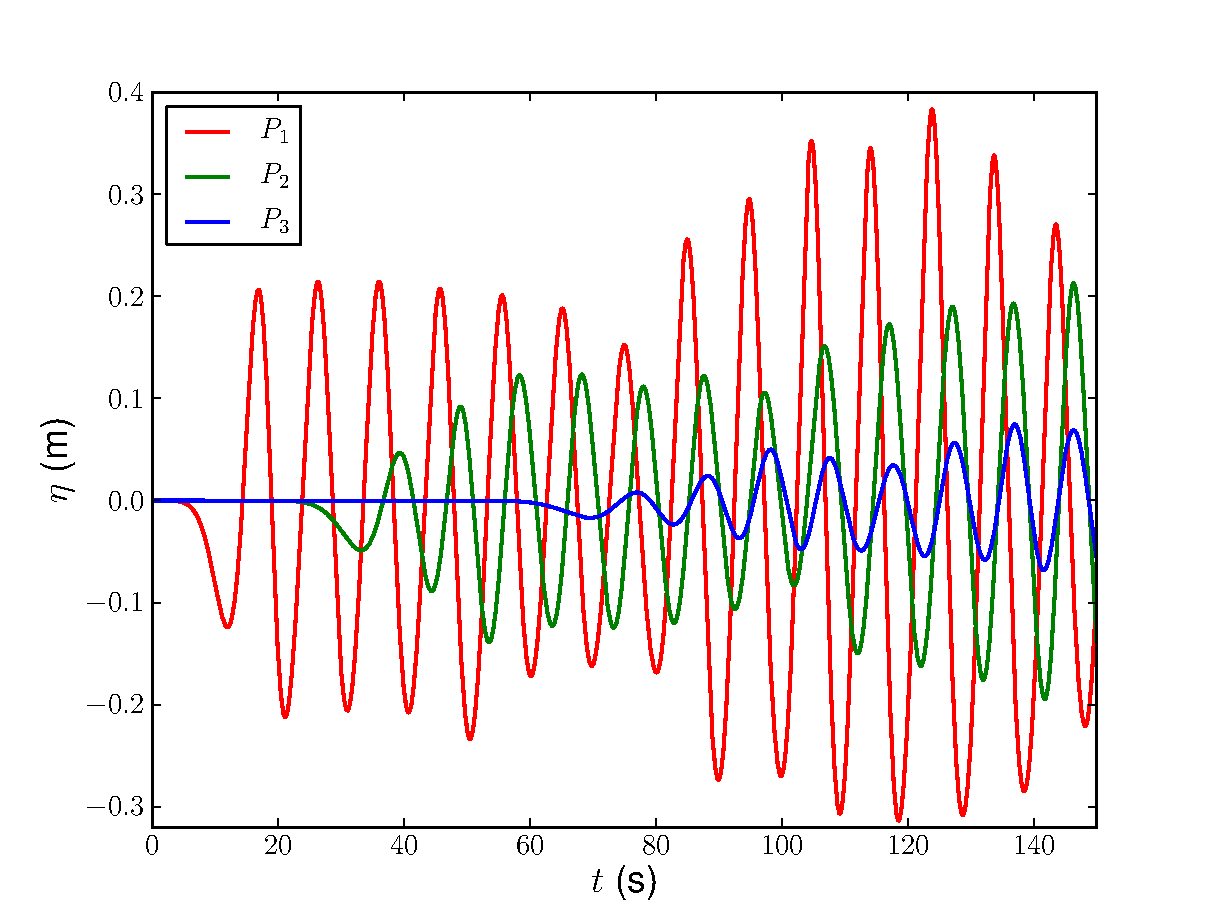
\includegraphics[width=\largefig]{chapters/lopes/pdf/etaprofile.pdf}
\end{center}
\caption{Wave surface elevation at $P_1$, $P_2$ and $P_3$ $[{\tt
      Max}\approx 0.4\, {\tt m}, {\tt min}\approx-0.31\,{\tt
      m}]$.}
\label{fig:lopes:etap}
\end{figure}
\begin{figure}
\begin{center}
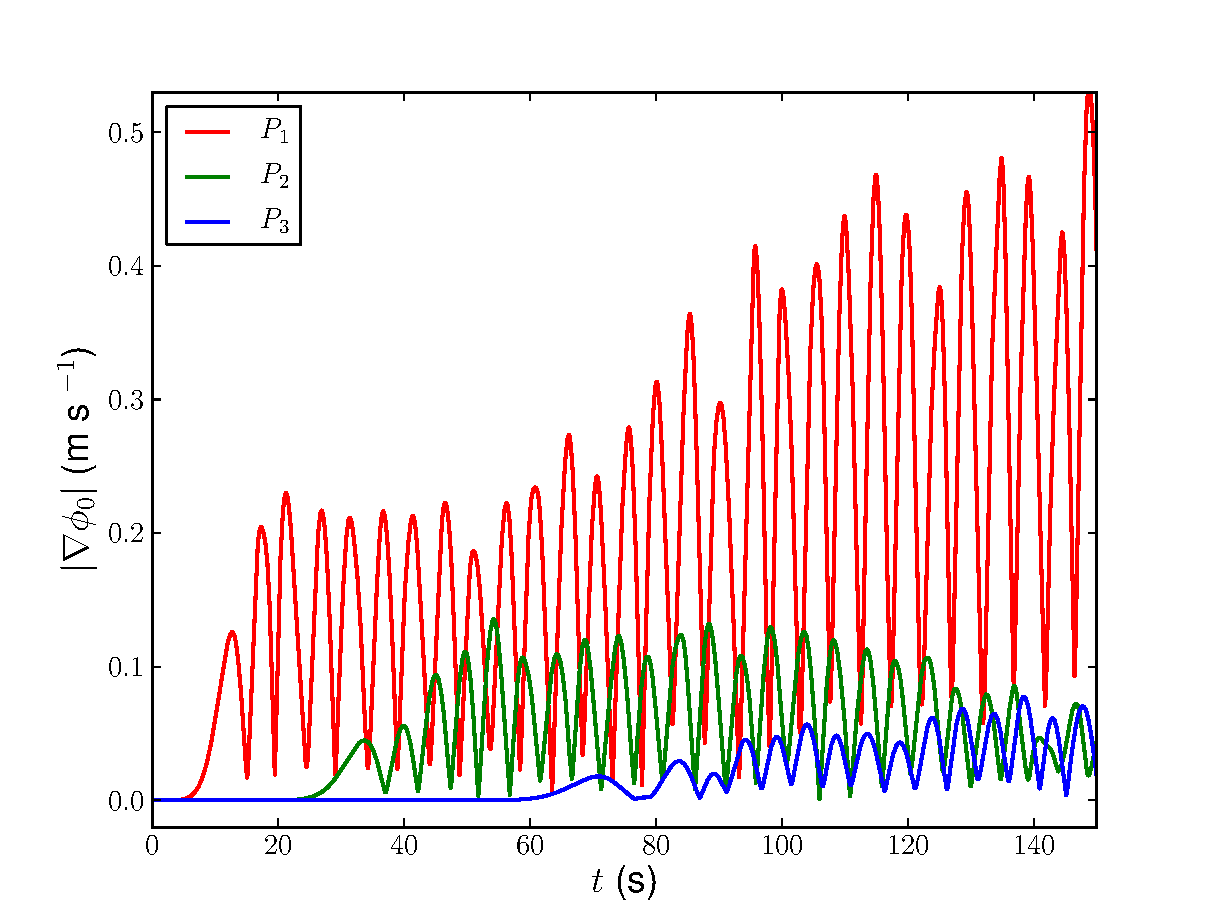
\includegraphics[width=\largefig]{chapters/lopes/pdf/velprofile.pdf}
\end{center}
\caption{Water speed at $P_1$, $P_2$ and $P_3$ $[{\tt
      Max}\approx 0.53\, {\tt m\, s}^{-1}, {\tt min}=0\,{\tt
      m\, s}^{-1}]$.}
\label{fig:lopes:velp}
\end{figure}

From these numerical results, we can conclude that the
interaction between incident and reflected waves, near the
harbor entrance, can generate waves with amplitudes that almost
take the triple value of the incident wave amplitude.  We
can also observe an analogous behavior for velocities.  Note
that no mechanism for releasing energy of the reflected
waves throughout the incident wave boundary is considered.


\subsection{Object moving on a horizontal bottom}
A wave generated by an object moving on a horizontal bottom
with a constant speed is simulated here.  The declaration of
the finite element discretization of
~\eqref{eq:lopes:varform} is that one described in
section~\ref{sec:lopes:numericalmethods}.

The spatial numerical domain is a rectangular basin of
$12.5\times 6\, {\tt m}^2$ discretized with a symmetric
uniform mesh with 2100 elements.  Full reflective boundary
conditions are only considered here.  The moving bottom $h\,
({\tt m})$ with a constant speed $S_0=1\, {\tt m\, s}^{-1}$
is defined by
\begin{equation}\label{eq:lopes:bottom1}
h(x,y,t)=0.45-\frac{\Delta h}{(1+\tanh(1))^4}{\bar
  X}(x,t){\bar Y}(y)
\end{equation}
with
\begin{equation}
{\bar X}(x,t)=(1+\tanh(2(x-x_l(t))))(1-\tanh(2(x-x_r(t)))),
\end{equation}
\begin{equation}
{\bar Y}(y)=(1+\tanh(2y+1)))(1-\tanh(2y-1)),
\end{equation}
\begin{equation}\label{eq:lopes:bottom4}
x_l(t)=x_c(t)-\frac{1}{2},\quad
x_r(t)=x_c(t)+\frac{1}{2},\quad x_c(t)=x_0+S_0t,
\end{equation}
 where $x_0=0\, {\tt m}$ and $\Delta h=0.045\, {\tt m}$ is the maximum
 thickness of the slide (see
 Figs. \ref{fig:lopes:objectbottom}--\ref{fig:lopes:objectbottom2}).
\begin{figure}
\begin{center}
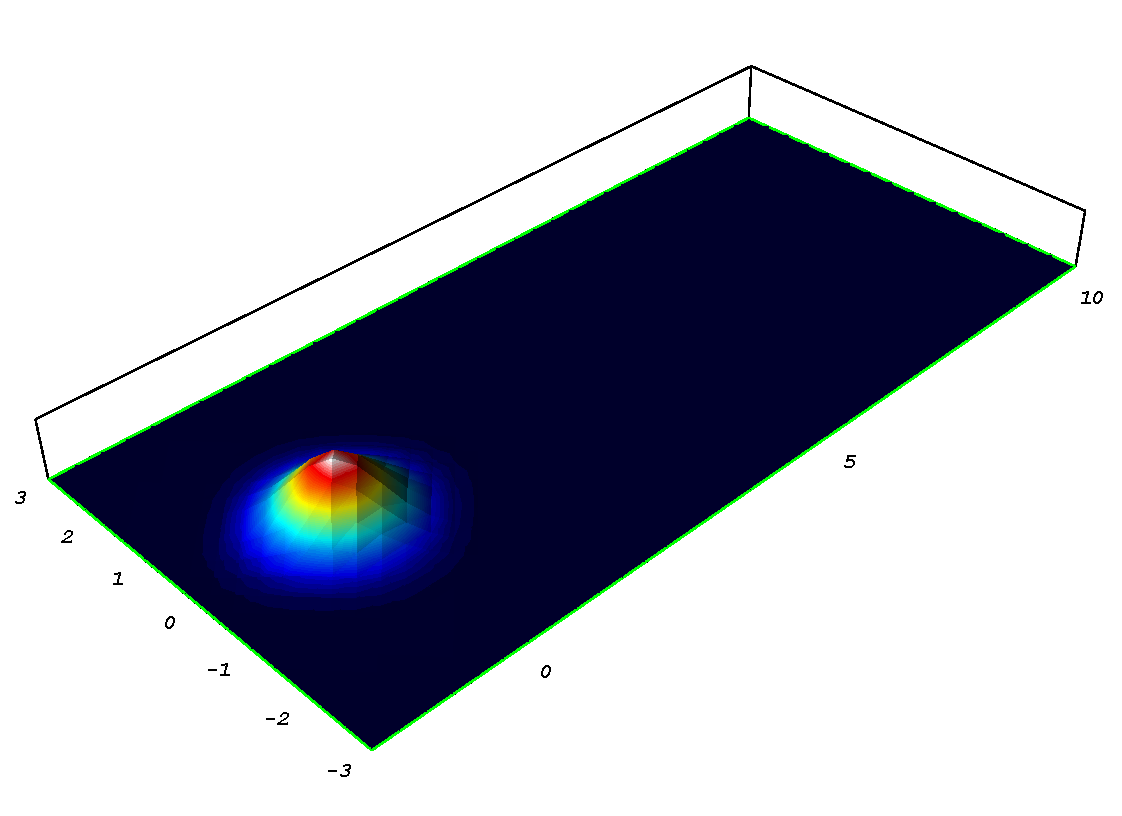
\includegraphics[width=\largefig]{chapters/lopes/pdf/depth0.pdf}
\end{center}
\caption{The impermeable bottom $-h(x,y,t)$ (m) at
  the time $t_0=0$ s. $[{\tt Max}= -0.405\, {\tt m},
    {\tt min}=-0.45\,{\tt m}]$}
\label{fig:lopes:objectbottom}
\end{figure}
\begin{figure}
\begin{center}
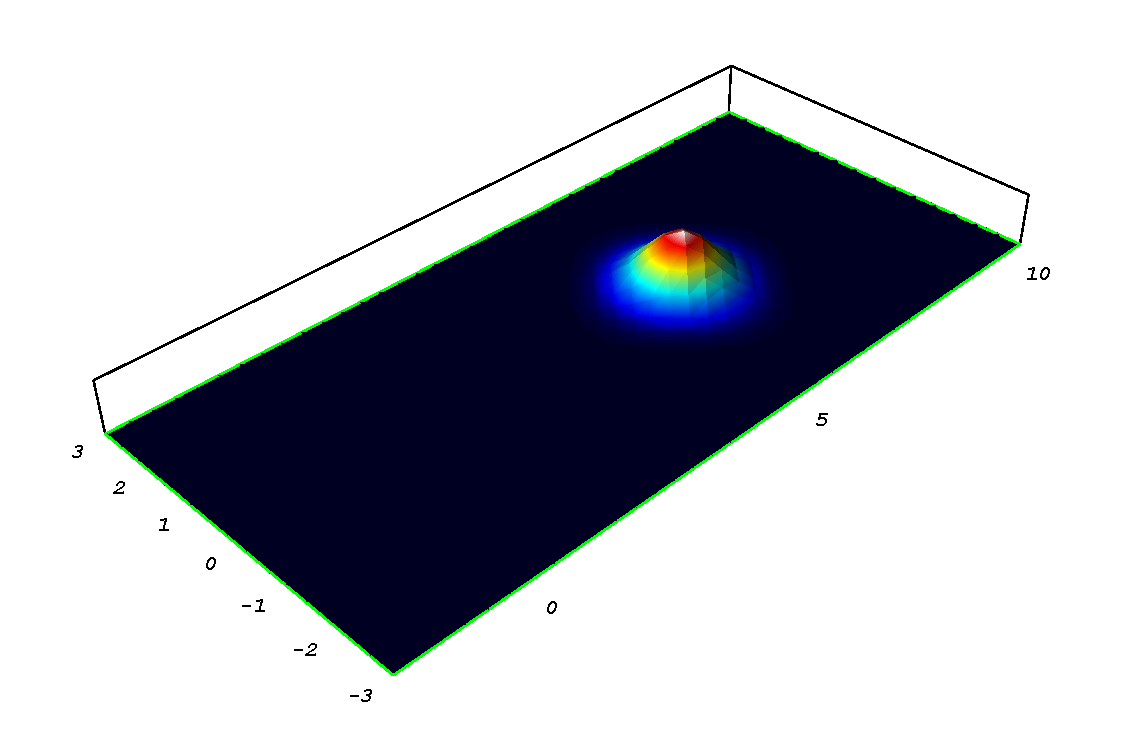
\includegraphics[width=\largefig]{chapters/lopes/pdf/depth6.pdf}
\end{center}
\caption{The impermeable bottom $-h(x,y,t)$ (m) at the time
  $t_2=6$ s. $[{\tt Max}= -0.405\, {\tt m}, {\tt
      min}=-0.45\,{\tt m}]$}
\label{fig:lopes:objectbottom2}
\end{figure}

A time step of $\Delta t=0.0005\, {\tt s}$ is considered.  In
Figs. \ref{fig:lopes:objectsurface0}--\ref{fig:lopes:objectsurface3},
we show four snapshots of the wave surface elevation
provided by the extended ZTC model at the time $t_0=1\, {\tt s}$, $t_1=3\, {\tt s}$,
$t_2=4.5\, {\tt s}$ and $t_3=6\, {\tt s}$.
Note that we also use here the color scale presented in Fig.~\ref{fig:lopes:scale}.
\begin{figure}
\begin{center}
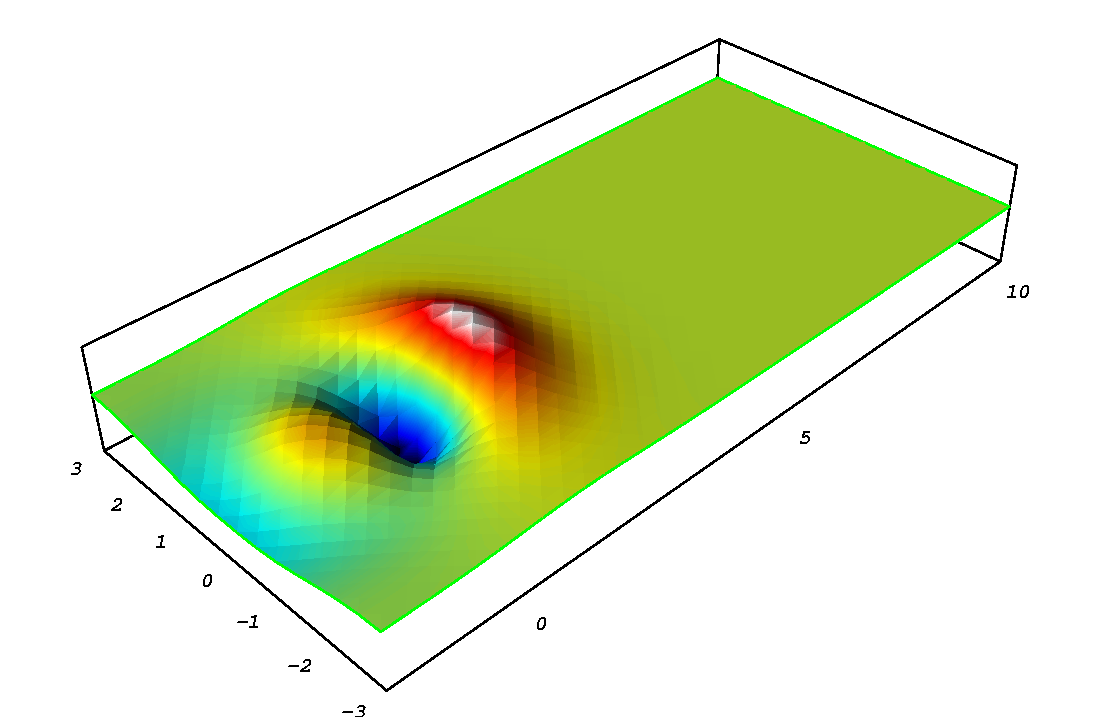
\includegraphics[width=\largefig]{chapters/lopes/pdf/eta1.pdf}
\caption{The  wave surface elevation $\eta$ (m) at the time
  $t_0=1$ s. $[{\tt Max}\approx 0.007\, {\tt m},
    {\tt min}\approx-0.010\,{\tt m}]$}
\label{fig:lopes:objectsurface0}
\end{center}
\end{figure}
\begin{figure}
\begin{center}
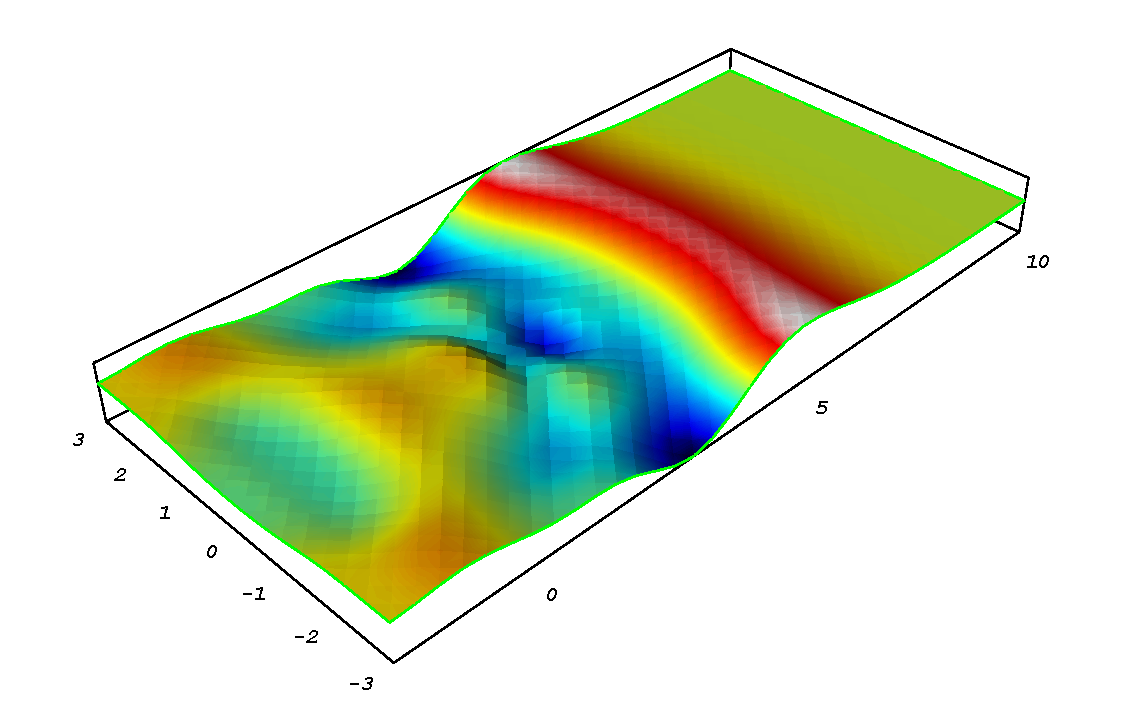
\includegraphics[width=\largefig]{chapters/lopes/pdf/eta3.pdf}
\caption{The  wave surface elevation $\eta$ (m) at the time
  $t_1=3$ s. $[{\tt Max}\approx 0.004\, {\tt m},
    {\tt min}\approx -0.006\, {\tt m}]$}
\label{fig:lopes:objectsurface1}
\end{center}
\end{figure}
\begin{figure}
\begin{center}
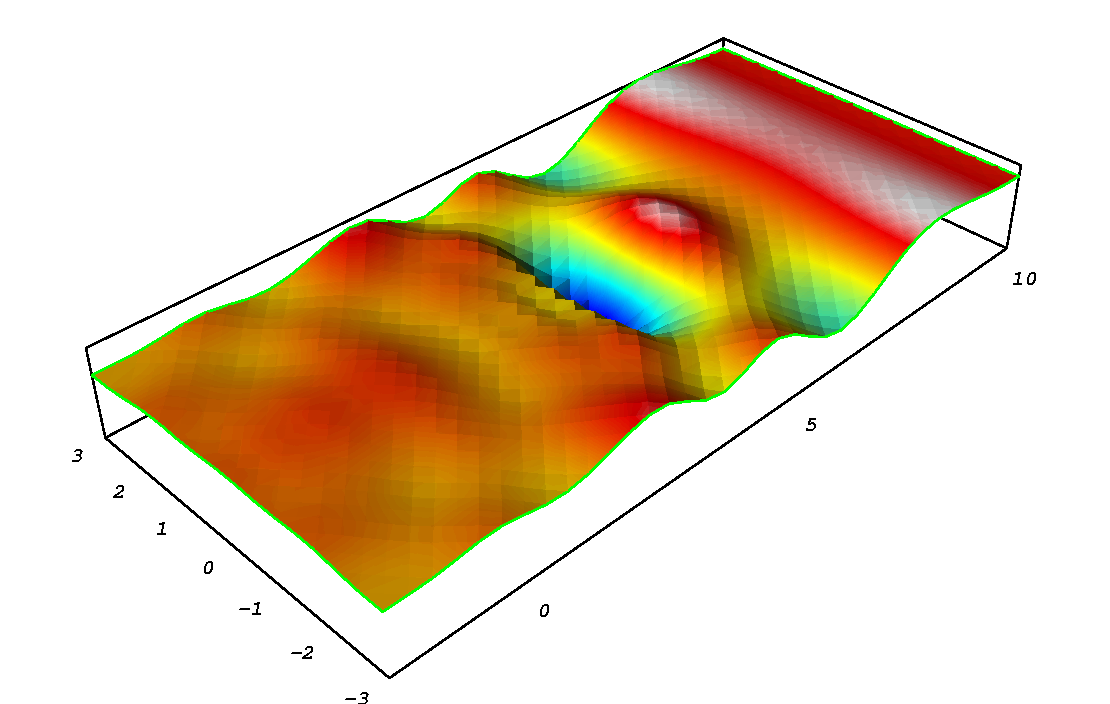
\includegraphics[width=\largefig]{chapters/lopes/pdf/eta45.pdf}
\caption{The wave surface elevation $\eta$ (m)
   at the time  $t_2=4.5$ s. $[{\tt Max}\approx 0.004\, {\tt m},
    {\tt min}\approx-0.011\, {\tt m}]$}
\label{fig:lopes:objectsurface2}
\end{center}
\end{figure}
\begin{figure}
\begin{center}
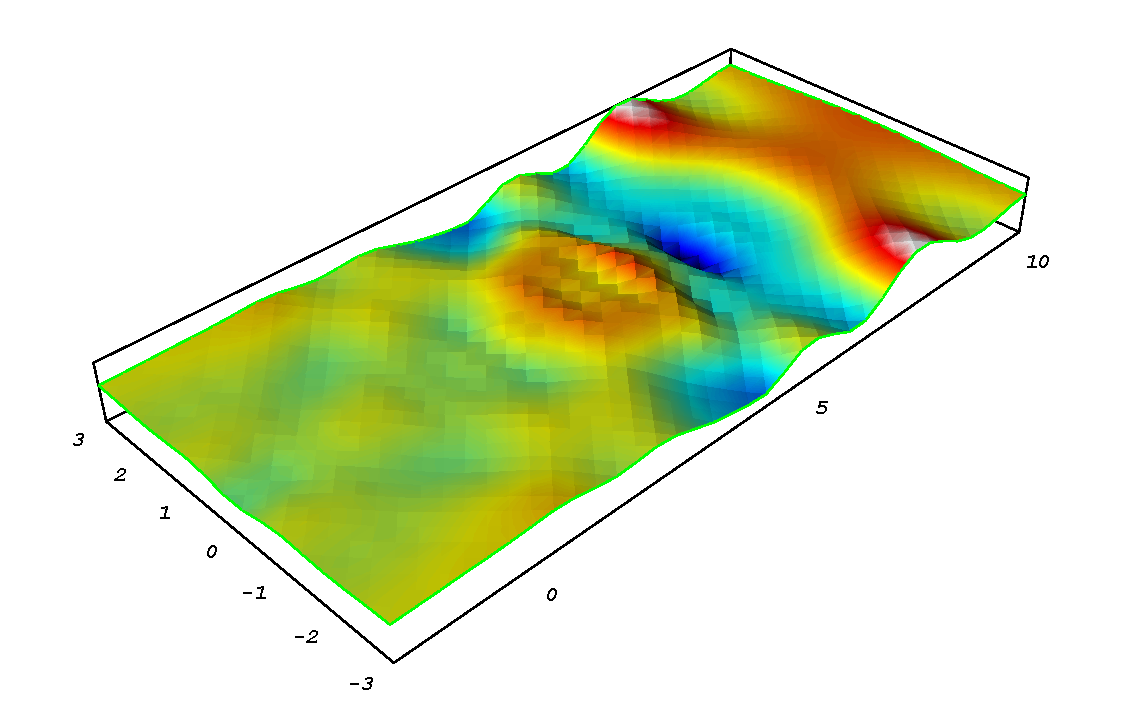
\includegraphics[width=\largefig]{chapters/lopes/pdf/eta6.pdf}
\caption{The  wave surface elevation $\eta$ (m)
   at the time  $t_3=6$ s. $[{\tt Max}\approx 0.004\, {\tt m},
    {\tt min}\approx -0.006\,{\tt m}]$}
\label{fig:lopes:objectsurface3}
\end{center}
\end{figure}

We refer that the bottom function given
by~\eqref{eq:lopes:bottom1}--\eqref{eq:lopes:bottom4} is not
piecewise linear. In fact, the spatial derivative functions
of any order obtained from $h$ are nonzero. Although the
extended ZTC model is based on a slowly varying bottom
assumption (only $O(h,\nabla h)$ terms are admitted), a good
agreement among the solutions presented here with those
provided by other models is achieved (see {\tt
  dolfwave/demo/2HD/horizontalLandslide}).  These other
models include $O(h,\nabla h,\nabla^2 h)$ terms
(see~\cite{LopesPereiraTrabucho}).
%}}}
\newpage
%{{{ Conclusions and future work
\section{Conclusions and future work}
As far as we know, the finite element method is not often
applied in surface water wave models based on the BEP
formulation.  In general, finite difference methods are
preferred, since they could be easily applied to equations
containing spatial derivatives with order higher than 2.  On
the other hand, they are not appropriate for the treatment
of complex geometries, like those of harbors, for instance.

In this work, we extend the BEP model
of~\cite{ZhaoTengCheng2004} in order to include dissipative
and surface tension effects, as well as, several types of
wave generation mechanisms, namely, by moving an impermeable
bottom or by the inclusion of a source function.  Moreover,
we study the influence of a dissipative term in the
dispersion properties, specifically, in the phase velocity.
We show the existence of some cutoff values for the wave
number such that the short length waves do not propagate.

The extended ZTC equations are used to model three different
physical problems: the evolution of a solitary wave passing
through a submerged bar; the evolution of a periodic wave in
a harbor and the generation of a wave due to an object
moving on a horizontal bottom.  These equations are
discretized using Lagrange $P_1$ elements and a
predictor-corrector scheme with an initialization provided
by an explicit Runge--Kutta method for the time integration.
In the first physical problem, we can conclude that the
numerical model is also stable when there is an interaction
between the incident and reflected waves over the submerged
bar as well as in one of the domain walls. The shoaling
effect over the submerged bar is clearly observed, both for
the incident and reflected waves.  In the harbor problem, we
remark that the interaction between incident and reflected
waves, near the harbor entrance, can generate waves with
amplitudes and velocities that almost take the triple values
of those observed in the incident waves.  In the last
numerical example, we refer that front wave generated by the
moving object travels faster than the object.  In this way,
a subcritical velocity regime associated with the moving
object is observed.  A good agreement among the numerical
solutions presented here with those provided by other models
is achieved (see {\tt dolfwave/demo}).  From these numerical
tests we can conclude that the \fenics packages,
namely \dolfin, \ufl and \ffc, are appropriate to model
surface water waves, leading to efficient and robust
algorithms.

Surface water wave problems are associated with
Boussinesq-type governing equations, which require high
order spatial derivatives. A first approach to a
fourth-order spatial derivative model, using a
continuous/discontinuous Galerkin finite element method, can
be found in~\cite{LopesPereiraTrabucho}.

We have been developing DOLFWAVE, i.e., a \fenics based
application for surface water wave models (see {\tt
http://www.fenicsproject.org/wiki/DOLFWAVE}).  This package
already includes some models with equations containing
spatial derivatives of order $4$.  The current state of the
work, along with several nume\-ri\-cal simulations, can be found
at {\tt http://ptmat.fc.ul.pt/$\sim$ndl} and {\tt
https://launchpad.net/dolfwave}.

As future work we are interested to include in DOLFWAVE
multilayer BEP models and investigate wave generation due to
time dependent finite element domains.
%}}}

